%% Copyright 2009 Elsevier Ltd
%%
%% This file is part of the 'Elsarticle Bundle'.
%% ---------------------------------------------
%%
%% It may be distributed under the conditions of the LaTeX Project Public
%% License, either version 1.2 of this license or (at your option) any
%% later version.  The latest version of this license is in
%%    http://www.latex-project.org/lppl.txt
%% and version 1.2 or later is part of all distributions of LaTeX
%% version 1999/12/01 or later.
%%
%% Template article for Elsevier's document class `elsarticle'
%% with numbered style bibliographic references
%%
%% $Id: elsarticle-template-1-num.tex 149 2009-10-08 05:01:15Z rishi $
%% $URL: http://lenova.river-valley.com/svn/elsbst/trunk/elsarticle-template-1-num.tex $
%%
\documentclass[preprint,12pt]{elsarticle}

\usepackage{isotope} % \isotope command
\usepackage{cleveref}
\usepackage{tabularx}

\usepackage{amsmath}
\usepackage{cleveref}
\usepackage{amssymb}
\usepackage{booktabs}
\usepackage{makecell}
\usepackage{multirow}
\usepackage[inline]{enumitem}
\usepackage{pgfplots}
\usepackage{pgfplotstable}
\usepackage[nowatermark]{fixmetodonotes}
\usepackage{comment}
\usepackage{siunitx}
% Use an ordinary space between a number and its associated unit
\sisetup{number-unit-product=\ }
% Start grouping digits into threes (with a space separator) for any
% number with four or more digits
\sisetup{group-minimum-digits = 4}
% Always express uncertainties as a separate number (not parenthesized digits)
\sisetup{separate-uncertainty = true}
% Don't use a space between a number and the percent sign
\DeclareSIUnit[number-unit-product = ]\percent{\char`\%}
% Custom units for this paper
\DeclareSIUnit\foot{ft}
\DeclareSIUnit\inch{inch}
\DeclareSIUnit\pot{POT}
\DeclareSIUnit\year{years}
\DeclareSIUnit\ADC{ADC\ counts}
\DeclareSIUnit\spill{spill}
\DeclareSIUnit\ton{t}



%% Use the option review to obtain double line spacing
%% \documentclass[preprint,review,12pt]{elsarticle}

%% Use the options 1p,twocolumn; 3p; 3p,twocolumn; 5p; or 5p,twocolumn
%% for a journal layout:
%% \documentclass[final,1p,times]{elsarticle}
%% \documentclass[final,1p,times,twocolumn]{elsarticle}
%% \documentclass[final,3p,times]{elsarticle}
%% \documentclass[final,3p,times,twocolumn]{elsarticle}
%% \documentclass[final,5p,times]{elsarticle}
%% \documentclass[final,5p,times,twocolumn]{elsarticle}

%% The graphicx package provides the includegraphics command.
\usepackage{graphicx}

%% The amsthm package provides extended theorem environments
%% \usepackage{amsthm}

%% The lineno packages adds line numbers. Start line numbering with
%% \begin{linenumbers}, end it with \end{linenumbers}. Or switch it on
%% for the whole article with \linenumbers after \end{frontmatter}.
\usepackage{lineno}

%% natbib.sty is loaded by default. However, natbib options can be
%% provided with \biboptions{...} command. Following options are
%% valid:

%%   round  -  round parentheses are used (default)
%%   square -  square brackets are used   [option]
%%   curly  -  curly braces are used      {option}
%%   angle  -  angle brackets are used    <option>
%%   semicolon  -  multiple citations separated by semi-colon
%%   colon  - same as semicolon, an earlier confusion
%%   comma  -  separated by comma
%%   numbers-  selects numerical citations
%%   super  -  numerical citations as superscripts
%%   sort   -  sorts multiple citations according to order in ref. list
%%   sort&compress   -  like sort, but also compresses numerical citations
%%   compress - compresses without sorting
%%
%% \biboptions{comma,round}

% \biboptions{}

\journal{Journal Name}

\begin{document}

\begin{frontmatter}

%% Title, authors and addresses

\title{Energy and Flavor Discrimination Using Precision Time Structure in On-Axis Neutrino Beams}

%% use the tnoteref command within \title for footnotes;
%% use the tnotetext command for the associated footnote;
%% use the fnref command within \author or \address for footnotes;
%% use the fntext command for the associated footnote;
%% use the corref command within \author for corresponding author footnotes;
%% use the cortext command for the associated footnote;
%% use the ead command for the email address,
%% and the form \ead[url] for the home page:
%%
%% \title{Title\tnoteref{label1}}
%% \tnotetext[label1]{}
%% \author{Name\corref{cor1}\fnref{label2}}
%% \ead{email address}
%% \ead[url]{home page}
%% \fntext[label2]{}
%% \cortext[cor1]{}
%% \address{Address\fnref{label3}}
%% \fntext[label3]{}


\def\LAPPDTM{LAPPD\textsuperscript{TM}~}
\def\LAPPDTMs{LAPPD\textsuperscript{TM}s~}
\newcommand{\Kzero}{\mbox{$\rm K^{0}$~}}

%% use optional labels to link authors explicitly to addresses:
%% \author[label1,label2]{<author name>}
%% \address[label1]{<address>}
%% \address[label2]{<address>}

\author{Evan Angelico [UofC], Andrey Elagin[UofC], Jonathan Eisch[ISU], Henry Frisch[UofC], Sergei Nagaitsev[Fermilab,UofC], Matthew Wetstein[ISU]}
\address[UofC]{Enrico Fermi Institute, University of Chicago, Chicago IL 60637}
\address[Fermilab]{Fermi National Laboratory, Batavia IL 60510}
\address[ISU]{Matt to Fill in}

\begin{abstract}
%% Text of abstract
We propose to use a higher-frequency RF structure and a small array of
photodetectors with time resolution of order 10-20 psec for muon
monitoring downstream of the decay volume to correlate neutrino interactions in both near and far on-axis detectors with the energy and flavor of each event. Analyses by the MINOS and MiniBooNE collaborations have previously looked at detailed features in the arrival time of neutrino bunches. Improving the capability to time scales of order 100 psec would allow selecting different neutrino energy and flavor spectra based on the arrival time of the neutrinos relative to the parent proton bunch time. Later neutrinos correspond to slower, and therefore lower energy, parent hadrons. In addition the fractions of tau, muon, and electron neutrinos and antineutrinos varies with the arrival time. The discrimination is currently limited by the bunch size of the protons impinging on the target.  We show that these effects can be resolved by measuring the pulse shape of each proton bunch using muon beam monitors with order 10-20 psec time resolution, and correlating the shape of each bunch with the localized wave front of the corresponding neutrinos as they traverse the detectors.  As opposed to off-axis experiments, which can only sample a small slice of the angular flux spectrum, this `stroboscopic' approach is analogous to sampling multiple off-axis angles with on-axis detectors, and applies equally to both near and far detectors in an oscillation experiment.
\end{abstract}



\begin{keyword}
Timing \sep Timing, Neutrino \sep Neutrino, Oscillation \sep Oscillation, RF-Structure \sep RF-Structure, Proton Bunch \sep Proton Bunch
%% keywords here, in the form: keyword \sep keyword
%% MSC codes here, in the form: \MSC code \sep code
%% or \MSC[2008] code \sep code (2000 is the default)

\end{keyword}

\end{frontmatter}

%%
%% Start line numbering here if you want
%%

\vskip-0.5in

\tableofcontents
\setcounter{tocdepth}{2} 

\newpage


\section{Introduction}
A deeper understanding of the neutrino sector, including CP violation,
the mass hierarchy, and deviations from unitarity of the PMNS matrix,
hinges on high precision, increasingly systematics-dominated
measurements of neutrino oscillation parameters. One approach to
reducing the systematic uncertainties is by expanding the range of L/E
and the mix of lepton family contributions measured simultaneously in
both near and far detectors. Here we present a scheme for such
measurements at Fermilab using the time-of-arrival of on-axis
neutrinos at the near and far detectors relative to the proton RF
structure.

The wide span of energies in neutrino beams stems from the wide range
of energies of the parent hadrons.  One technique for optimizing
the neutrino energy spectrum for measuring oscillations at a given
detector distance is to look at angles off-axis from the pointing of
the beam, a technique notably exploited by the NOvA and T2K
experiments.
% Matt is this correct?

An alternative method for understanding and selecting different energy
spectra within a neutrino beam exploits the differing velocities of
the parent hadrons. Lower energy pions and kaons travel more slowly,
especially as they approach sub-relativistic energies. As a
consequence, lower energy neutrinos are created further behind the rest of
the bunch. Selecting later arriving neutrinos would provide an
increasingly pure low-energy subset of the overall flux.\footnote{As shown
below, the time difference from hadron travel outweighs the compensating
effect that higher energy hadrons live longer.}

% Matt's sentences need referencing..
The idea of using timing to resolve beam structure has a long
history. Efforts to detect dark matter have relied on time-of-flight
differences between dark matter particles and neutrinos. In 1998
M. Goldhaber pointed out that neutrinos from SN1987A were detected
earlier in Kamiokande than in IMB due to the correlation of energy and
time of production~\cite{mgoldhaber}. The energy-dependent time
evolution of supernova neutrinos has also been proposed as a means of
determining the mass hierarchy~\cite{Supernova_time_hierarchy}. Timing
has been employed to identify a pure sample of stopped kaons and pions
in neutrino beams. Several notable efforts have utilized bunch timing
to place limits on neutrino velocity~\cite{opera_2011}. MINOS, in
particular, noted interesting kinematic relationships within the beam
time.

The MiniBooNE collaboration has recently explored the idea of using
timing relative to the RF structure of the proton beam 
to select on the neutrino energy spectrum. However, efforts to
select different energy spectra on the basis of beam timing have been
largely overlooked due to two considerations: (1) Limited time
resolutions of the detectors themselves were insufficient to see the
O(100) psec effect, and (2) the $\sim$900 psec spread of the proton
bunch impinging on the target washes out most of the effect. We
address both these issues below.

Here we revisit the idea of using beam timing to select different
energy components of the neutrino flux, but with a higher-frequency RF
structure superimposed on the proton beam after normal acceleration
but before extraction to make shorter proton bunches.

%\subsection{Organizational Outline}
An overview of the `stroboscopic' approach introduced above is
presented in Section~\ref{approach}. Section~\ref{Fermilab} describes
the outlines of a first implementation at Fermilab.
Section~\ref{mechanism} describes the mechanism of energy and flavor
separation by `time slicing' relative to the parent proton bunch
structure, and the impact of proton bunch size on the separation.
Section~\ref{time_sorted_spectra} presents energy spectra for
electron, muon, and tau neutrinos and anti-neutrinos for time windows
referenced to the their identified parent proton bunch.

Section~\ref{RF} addresses the accelerator and RF issues of rebunching
the protons at higher RF frequency, starting with the 53 MHz of the
Fermilab Main Injection. Bunch profiles are presented from simulations
of a 500 MHz Cornell RF cavity ramped up as the 53 MHz is ramped
down. Measuring the profile of each proton bunch relative to a precise
system clock using muons and a system of fast photodetectors is
described in Section~\ref{muon_monitor}.  Section~\ref{results}
summarizes the energy spectra for electron, muon, and tau neutrinos
and anti-neutrinos for the 500 MHz beam profiles of
Section~\ref{RF}. Conclusions and areas of needed development are
presented in Section~\ref{conclusions}.



%
% Section The Stroboscopic Approach}
%
\section{The Stroboscopic Approach}
\label{approach}
We have dubbed the time-slicing of neutrino events relative to the
time of their parent bunch as a 'stroboscopic' approach, as it is
essentially successive snapshots of the neutrino bunch but with
different energy spectra and different neutrino family populations in
each time bin. We describe the basic ingredients of the technique
below.

\subsection{Timing Relative to Wave Fronts of Zero Time At the Detector}
\label{wave_front}

The RF structure of the proton beam at the neutrino target imprints
the interaction rate on the production of the hadrons that are the
primary source of neutrinos, as indicated in
Figure~\ref{fig:wave_fronts}. The spacing of the waves is given by the
period of the RF structure on the proton beam, $\tau$. The width of
the wave front depends on both the width of the proton bunch in the RF
bucket convoluted with the difference in time between the
production of the parent hadrons  at the target and their subsequent
decay that produces the neutrinos. An additional factor is the
different path lengths of the parent hadrons through the neutrino
focusing horn and decay region. 

\begin{figure}[ht]
	\begin{center}
           	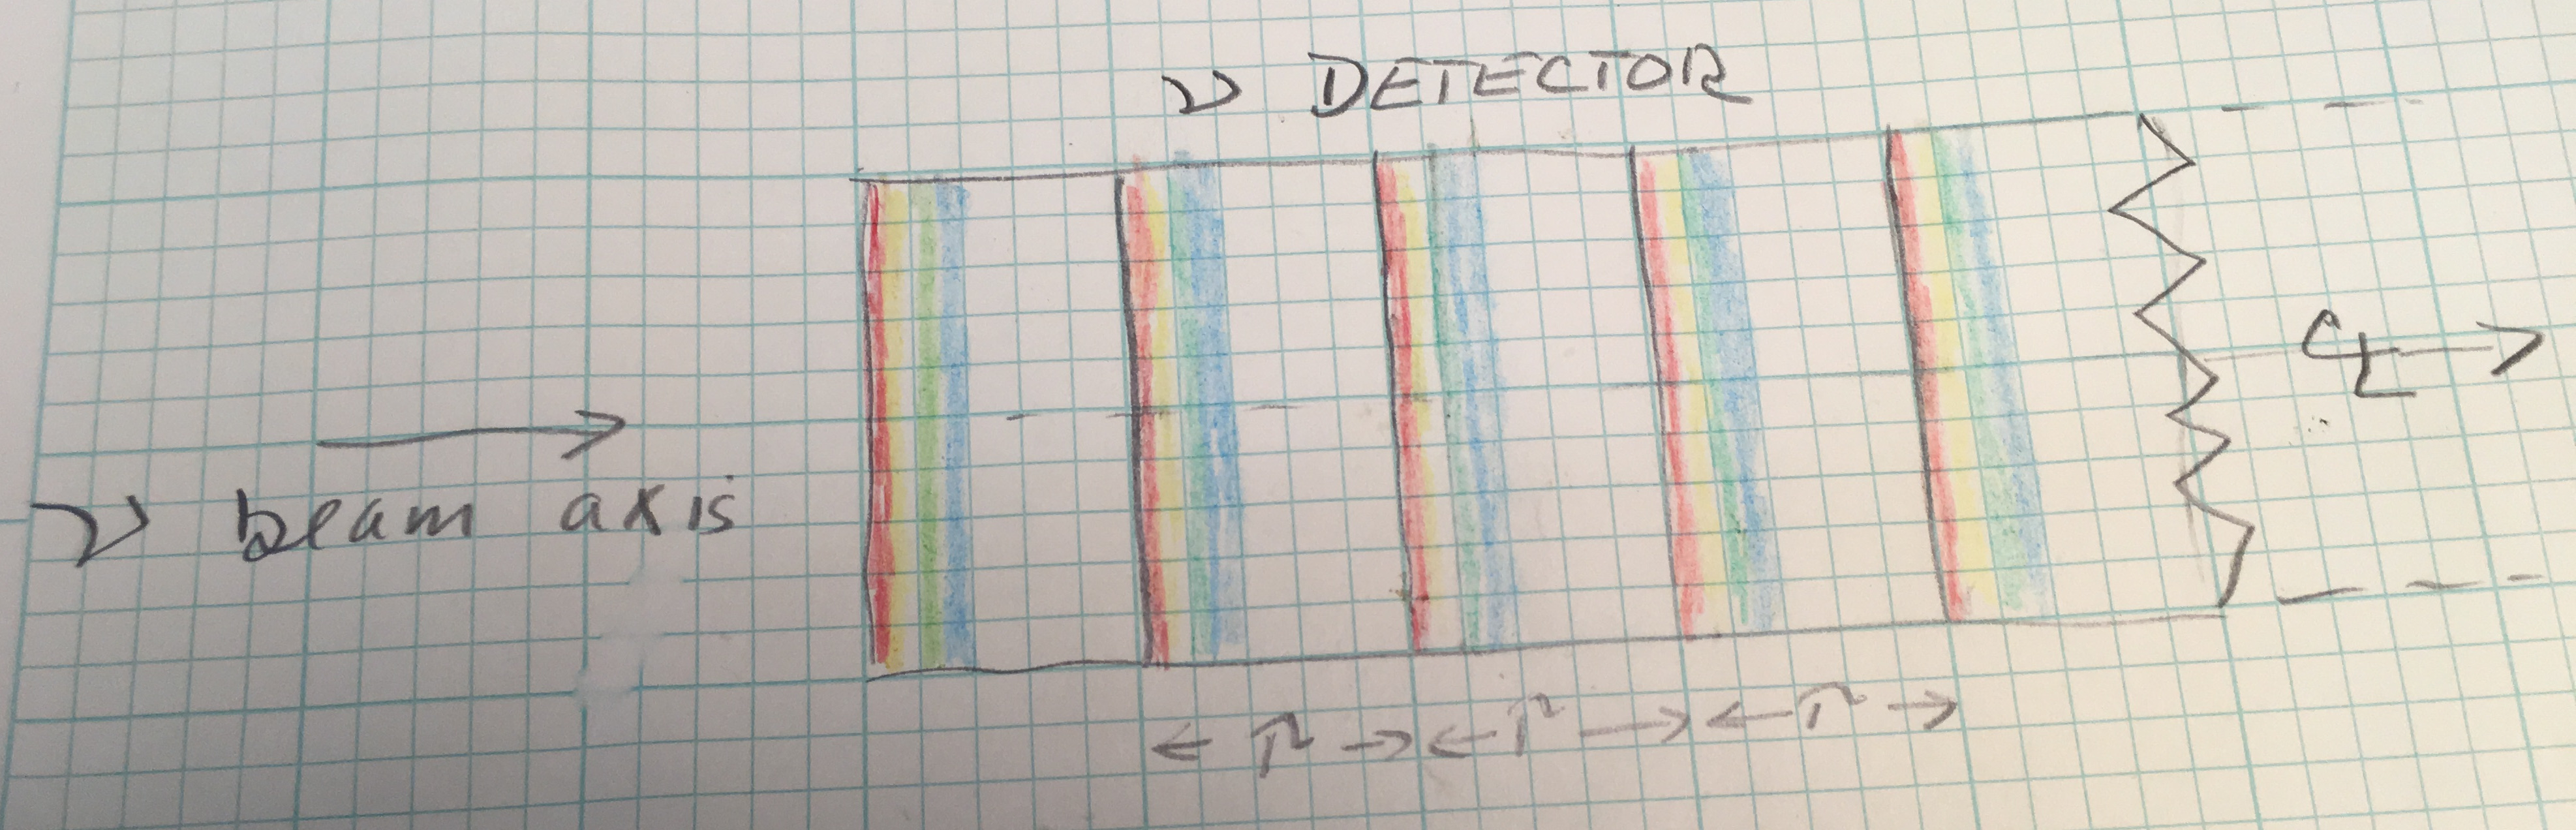
\includegraphics[width=1.0 \linewidth]{Figures/nupaper_waves_IMG_5834_crop.jpg}
	\end{center}
	\caption{A `snap-shot' of the neutrino wave-front moving
          through a neutrino detector.}

	\label{fig:wave_fronts}
\end{figure}



\subsection{Time Reference to Proton Bunch-by-Bunch Interaction
  Profiles at the Target}
\label{time_reference}

Figure~\ref{fig:bucket_timing} shows the time relationship between the
RF structure of the protons at the target and the neutrino events in a
detector at distance L from the target. The period of the RF is
denoted by $\tau$, and the FWHM of the proton bunch is denoted by
$\sigma_p$. Each neutrino bunch is offset to a later time from its
parent proton bunch by approximately $L/c$, where $c$ is the speed of
light.

The neutrinos from a given proton bunch arrive at the detector before
a signal can be transmitted using electromagnetism, i.e. real or
virtual photons. One consequently has to locally record the relevant
data on a bunch-to-bunch basis at the RF frequency. Each bunch should be
time stamped at both the target and the detector so that the data from
target and detector can be re-united
robustly. Section~\ref{muon_monitor} describes the muon monitor
systems that provide the data on the time profile of protons on target
for each bunch. 

\begin{figure}[ht]
	\begin{center}
           	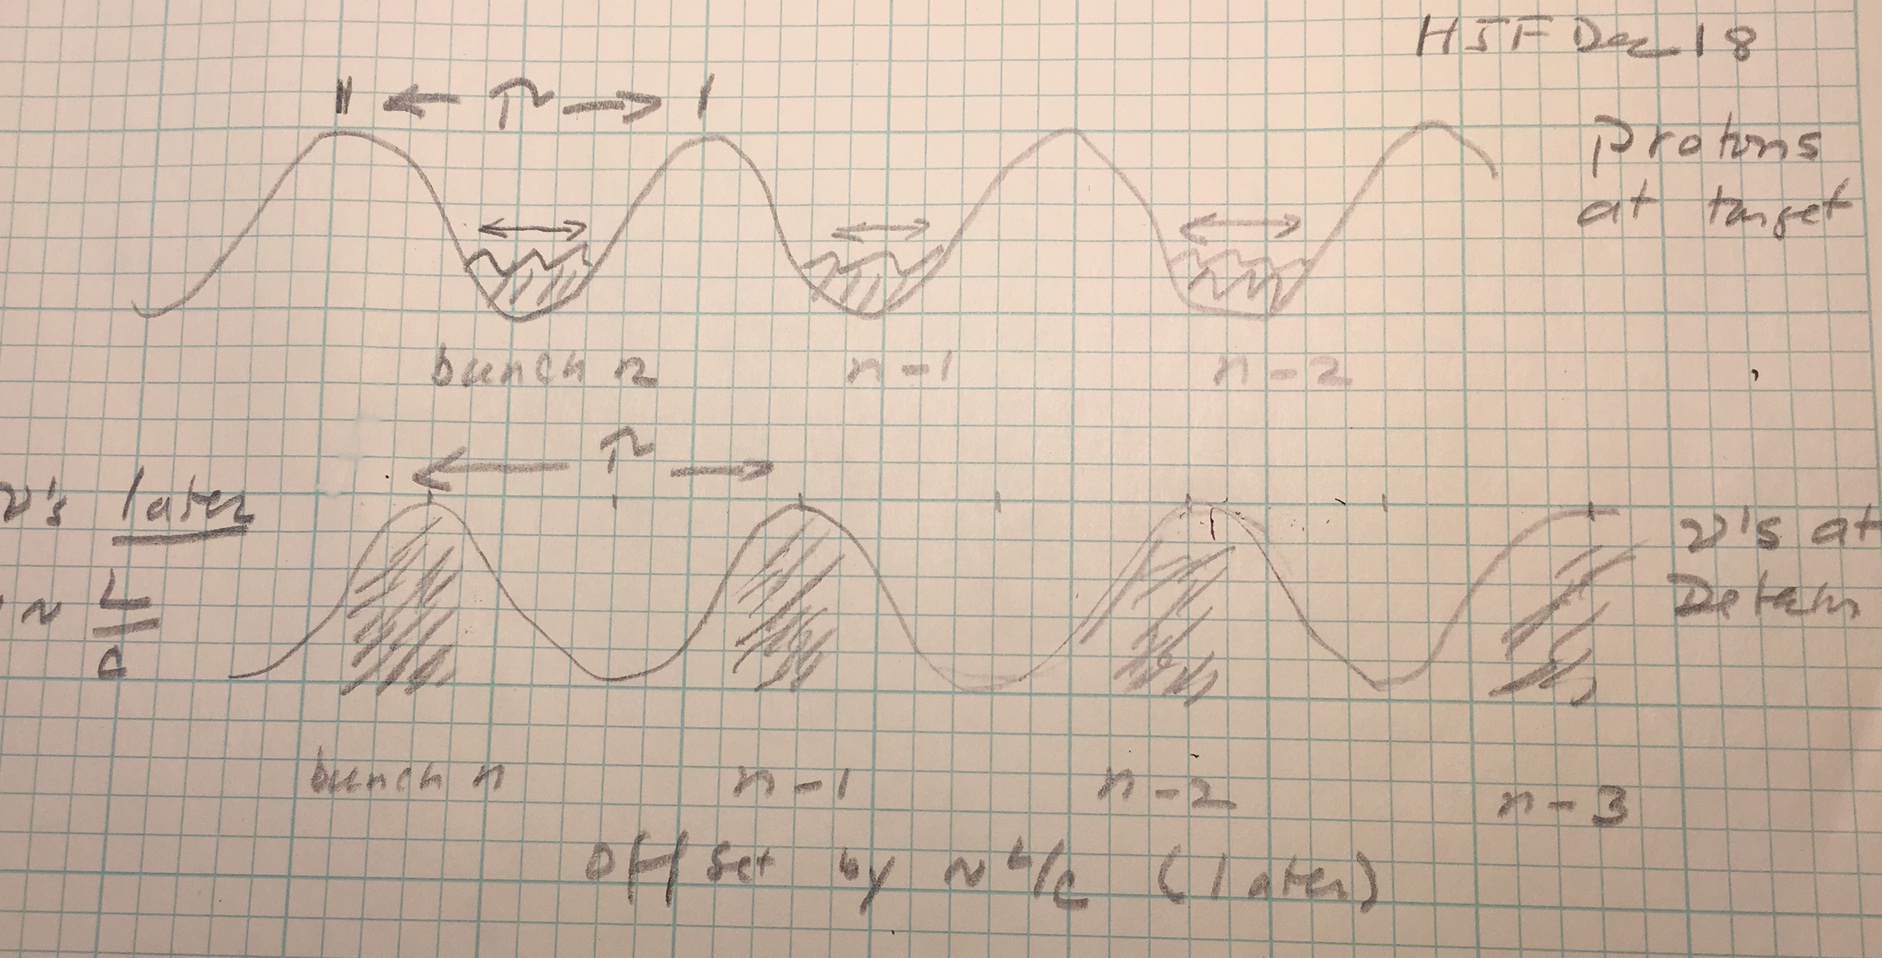
\includegraphics[width=0.7 \linewidth]{Figures/nupaper_timing_IMG_5836_crop.jpg}
	\end{center}
	\caption{A 'cartoon' of the correspondence bucket-by-bucket of
          the neutrino neutrino wave-front timing at the neutrino
          detector and the protons interacting with the target. The
          separation is given by the RF period $\tau$, and the FWHM of
        the proton bunch is denoted by $\sigma_p$.}
	\label{fig:bucket_timing}
\end{figure}

\subsection{Energy and Flavor Spectra Sorted by Time Slice Relative to
the Parent Proton Bunch}
\label{spectra}


Figure~\ref{fig:wave_fronts} also indicates the `stroboscopic' nature
of this proposal. Neutrinos from lower energy hadron parents
(indicated in red) arrive in a distribution that tends 
later than neutrinos from higher energy
parents (indicated in blue), as described below in
Section~\ref{mechanism}. Time-slicing relative to the specific parent 
proton  bunch, i.e. on
a bunch-to-bunch basis, produces different energy spectra in each
time-slice. The spectra will also depend on the family type of the
neutrino, as electrons and muons are produced in different rations
from pions and kaons, and tau neutrinos, while rare, will be
predominantly produced by short-lived parents.

% End Section 2


%
% Section Fermilab Neutrino Infrastructure
%
\section{Fermilab Neutrino Facilities}
\label{Fermilab}
The proposed `stroboscopic' scheme requires some modifications to the
current neutrino production facilities. A new RF cavity in the Fermilab Main
Injector at a higher harmonic of the 53 MHz to superimpose a
hyper-fine bunch structure on the protons, providing short enough
bunches, spaced widely enough to fully exploit the energy spreading
effect. Acceleration would be as currently done, followed by a
ramp-down of the 53 MHz with a concurrent ramp-up of the higher
harmonic. New muon monitors with precise time resolution would be
needed downstream and at 90$^o$ with respect to the target. Precision
clocks would be needed at both the detector and the target to
synchronize the RF bunches.  No time measurement is necessary at the
neutrino detectors, but the bunch profile synchronization will require DAQ
infrastructure to hold and match the two data streams from the target and
detector.


%
%YOUAREHERE

%\subsection{The Main Injector and the 53 MHz Accelerating RF}

Figure~\ref{fig:fermilab_facility_aerial} shows an aerial view of the
Fermilab Accelerator complex. The Main Injector (MI), shown in the
foreground, accelerates protons from their injection energy of 8 GeV 
to 120 GeV~\cite{units}, after which
they are extracted and directed onto the neutrino target. The
accelerating frequency at flat-top is 53.xxx MHz.

The typical MI cycle time~\cite{vaia} is xxx (1.2) seconds, with a
typical spill length of xxx (10?) $\mu$s. 
%We have imposed the
%requirement that the changes to the acceleration/extraction cycle
%required by a higher-frequency RF not
%lower the delivered intensity by more than 5\%.


\begin{figure}[ht]
	\begin{center}
           	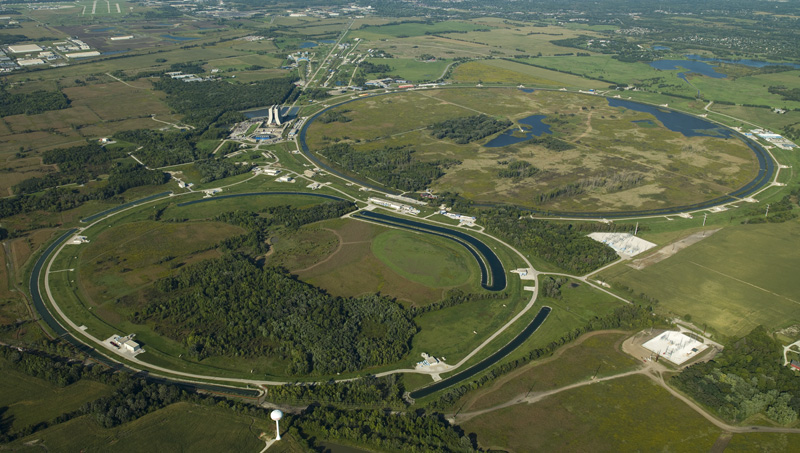
\includegraphics[width=0.7 \linewidth]{Figures/fermilab_facility_07-0329-14D.jpg}
	\end{center}
	\caption{An aerial view of the Fermilab Accelerator complex.
         The Main Injector, from which the protons are extracted onto
         the neutrino target, is in the foreground. (Credit: Fermilab)}
	\label{fig:fermilab_facility_aerial}
\end{figure}


%\subsection{Proton Target, Neutrino Horn, and Decay Volume}

Figure~\ref{fig:numi_horn} shows the layout of the Fermilab NUMI
neutrino production target, focusing horn, decay region (need to
remake the picture with no Minerva and showing 90 degree muons and FWMM). 


\begin{figure}[ht]
	\begin{center}
           	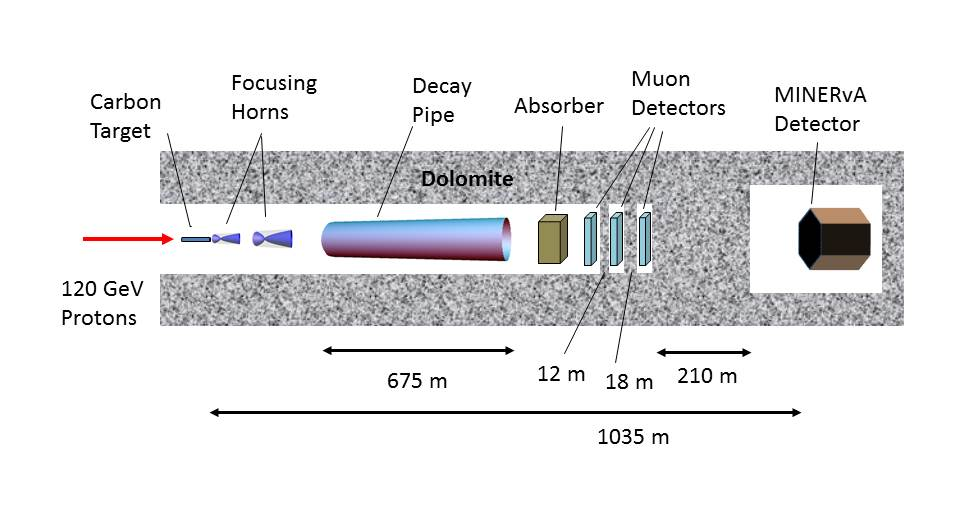
\includegraphics[width=1.0 \linewidth]{Figures/numi_horn_how_works.jpg}
	\end{center}
	\caption{The layout of the Fermilab NUMI neutrino production
          target, focusing horn, decay region, and the Minerva
          experiment. (Credit: Minerva) Needs to be remade no Minerva,
        with TRMM, FWMM}
	\label{fig:numi_horn}
\end{figure}



%\subsection{Properties of the Current Near and Far Detectors}

%\subsection{Constraints: Aperture, the Abort Gap, Radiation Losses, Proton-on-Target}

The proposed superposition of a higher-frequency RF on the current 53
MHz of the Main Injector is subject to several operational
constraints that have impact on the implementation. First, the
aperture of the higher-frequency RF cavity must be large enough not
to limit the MI aperture. Second, during the transition to higher
frequency the longitudinal loss into the abort gap needs to be less
than xxx. Radiation losses from other sources during the transition
must be acceptable. A loss of integrated protons-on-target (POT) due
to the increase in cycle time to accommodate the RF transition should
be small; we take 5\% as a nominal limit. Lastly, cost and schedule
indicate finding an existing hardware solution that can be purchased.

% End of Section 3



%\section{Energy and Flavor Separation By Time-of-Arrival}
\label{mechanism}

The power of this technique stems from the fact that, in contrast to
off-axis measurements, the different neutrino energy spectra can be
selected within the same detector. Moreover, these timing
relationships can be applied in near and far detector alike. 

We emphasize that the time of individual neutrino events is determined
by the position of the vertex with respect to the phase of the RF, and
requires no time measurement capability in the detector
itself. Instead, the RF
structure is measured bunch-by-bunch by a 10-15 GHz waveform sampling
system by the muon monitor system (MMS). The recorded stream of bunch 
structure parameters or profiles is time-stamped and synchronized with
the detector data as a separate operation.

\begin{figure}[t]
	\begin{center}
        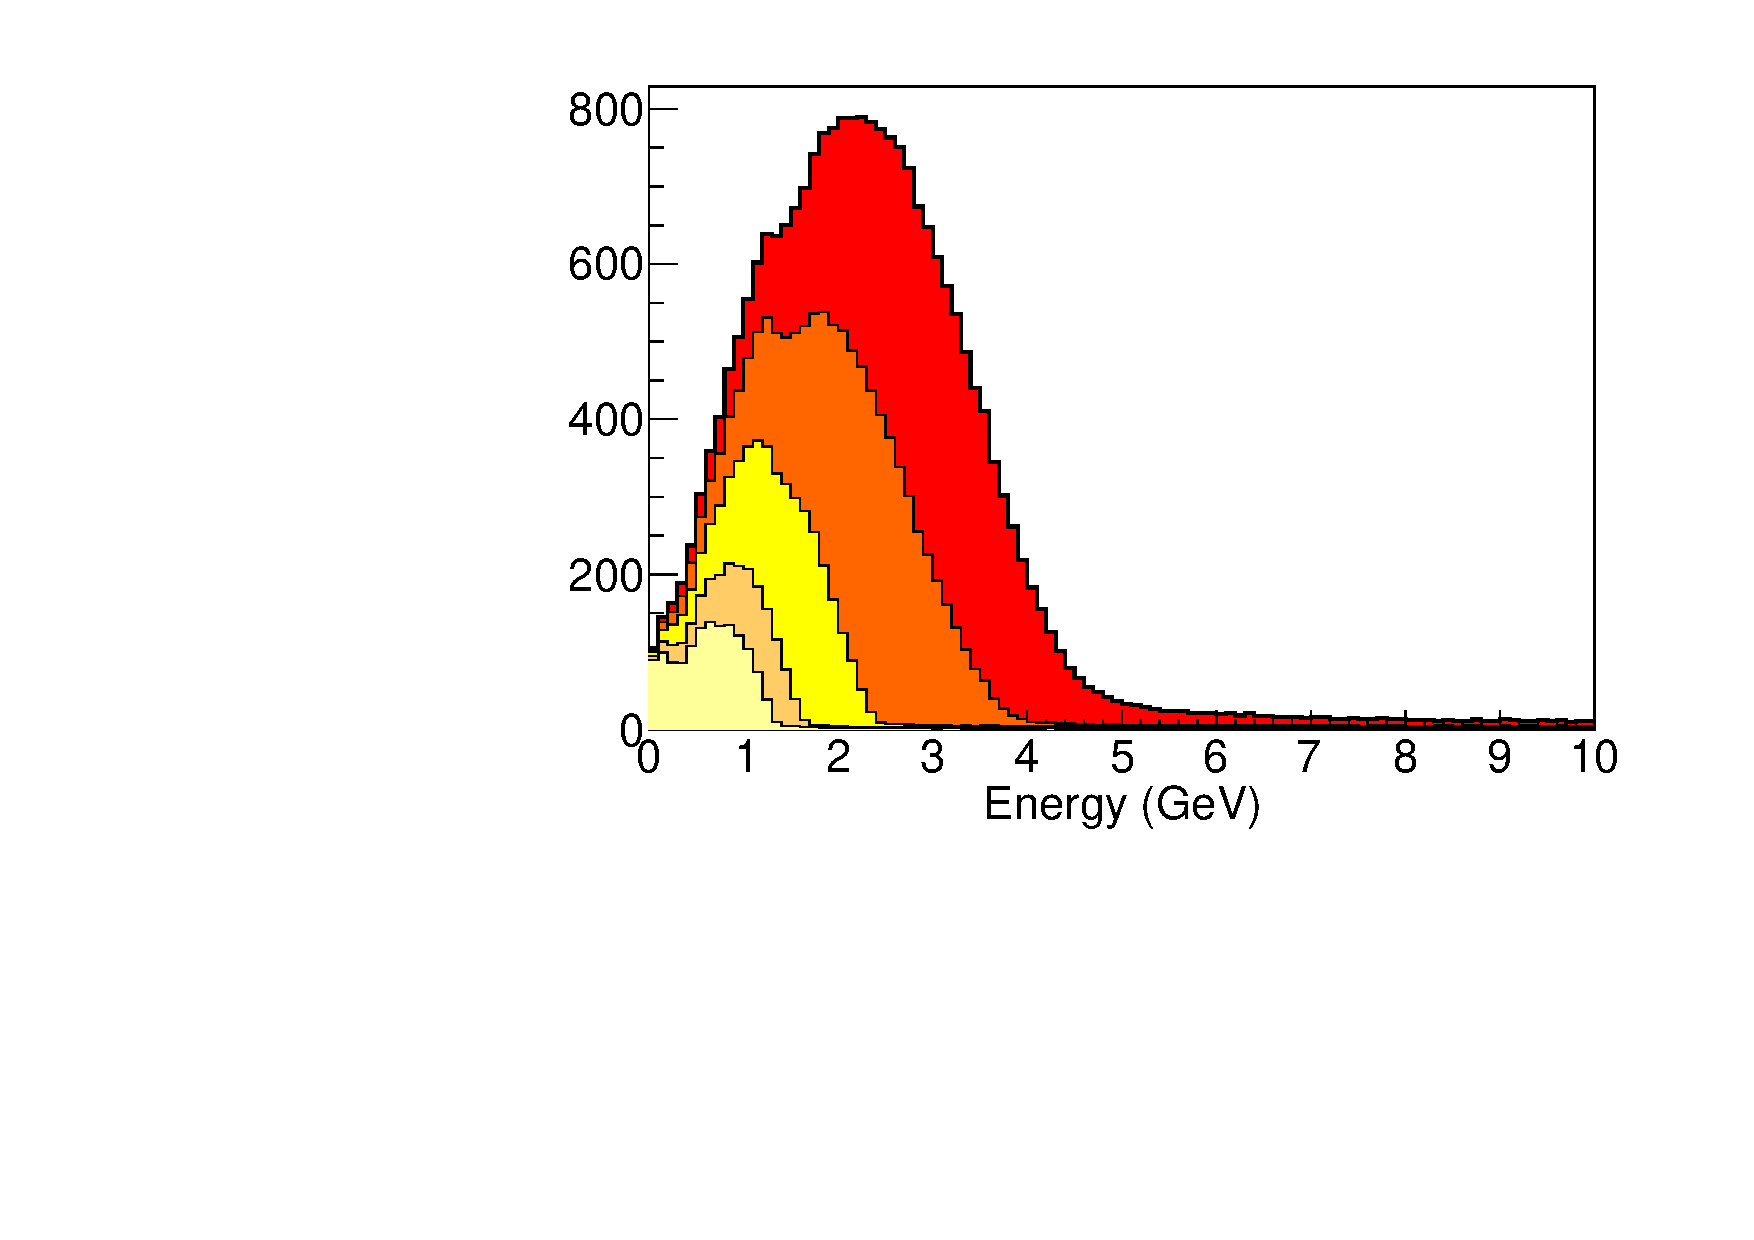
\includegraphics[width=0.5\linewidth]{Figures/DUNEbeam_truetimingB.pdf}
	\end{center}
	\caption{The DUNE forward horn current flux (red), with the
          fluxes corresponding to increasingly later time-cuts on the
          bunch time, assuming no time spread of the protons on
          target: 250 psec after the start of the neutrino bunch
          (orange), 500 psec after (yellow), 750 psec (dark beige), 1
          nsec (light beige).}
		\label{fig:Dunebeam_truetimingB}
\end{figure}


\begin{figure}[t]
	\begin{center}
           	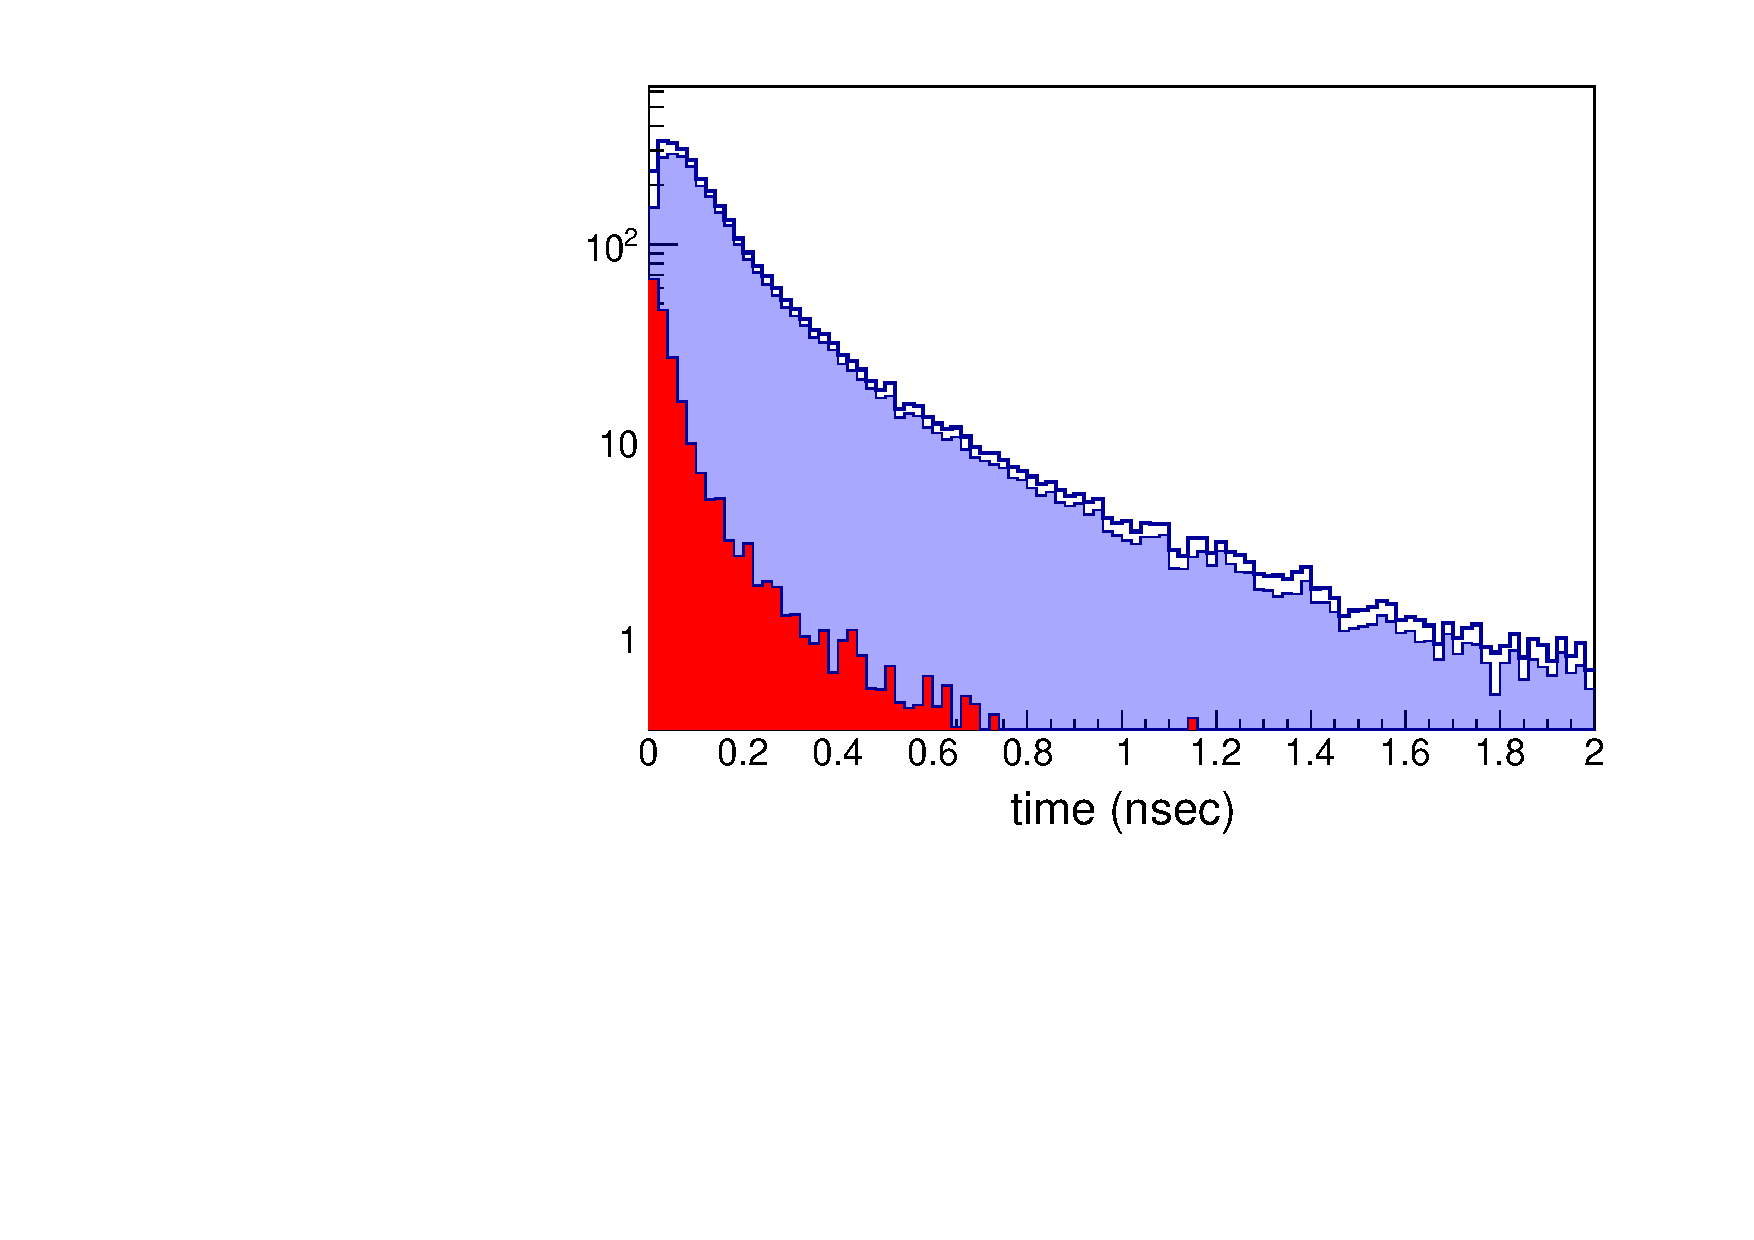
\includegraphics[width=0.5\linewidth]{Figures/RHCbeamcontent_log.pdf}
	\end{center}
	\caption{The time spectrum of anti-neutrinos in reverse horn
          current mode (blue) overlaid with wrong-sign neutrino
          contamination in red. The wrong-sign component drops off
          more quickly.}
		\label{fig:RHCbeamcontent_log}
\end{figure}

\subsection{Derivation of Time Dispersion}

The difference in arrival time of a neutrino from a sub-relativistic
pion of energy E' with respect to a high energy pion traveling with
speed $\sim$c is given by:

\begin{equation}
\Delta t(E') = \frac{c - v(E')}{c} \tau (E')
\end{equation}

Where $\tau (E')$ is the lifetime of the lower energy pion in the lab
frame. The time spreading will only occur until the decay of the lower
energy pion, at which point the daughter neutrinos will propagate at
c. The lifetime of the higher energy pion is irrelevant, since the
pion is already propagating at roughly c.

\begin{equation}
\Delta t(E') = \tau (E') [1 - \beta (E')]
\end{equation}

Rewriting in terms of the pion lifetime in the restframe, $\tau_0$, we get:

\begin{equation}
\Delta t(E') = \left(\frac{E'}{m} \tau_0\right) \left[1 - \sqrt{ 1 - \frac{m^2}{E'^2}} \right] 
\end{equation}

Regrouping the equation, we get the relationship:

\begin{equation}
\Delta t(E') = \left[\frac{E'}{m} - \sqrt{ \frac{E'^2}{m^2} - 1}\right] \tau_0
\label{eq:beamkinematicsandtiming}
\end{equation}

As one would expect, at the lowest energies, where the pion is
essentially at rest in the lab frame, $\Delta t(E')$ approaches the
lifetime of the pion in the rest frame, $\tau_0$. At high energies,
the speed of the lower-energy pion approaches that of the higher
energy pion and thus $\Delta t(E')$ goes to zero.

Figure~\ref{fig:beamkinematicsandtiming} shows a plot of
equation~\ref{eq:beamkinematicsandtiming} (TOP), and the simulated
relationship between $\Delta t(E')$ and E' for the DUNE beam.

\begin{figure}[h]
	\begin{center}
           	\begin{tabular}{c c}
 \multicolumn{2}{c}{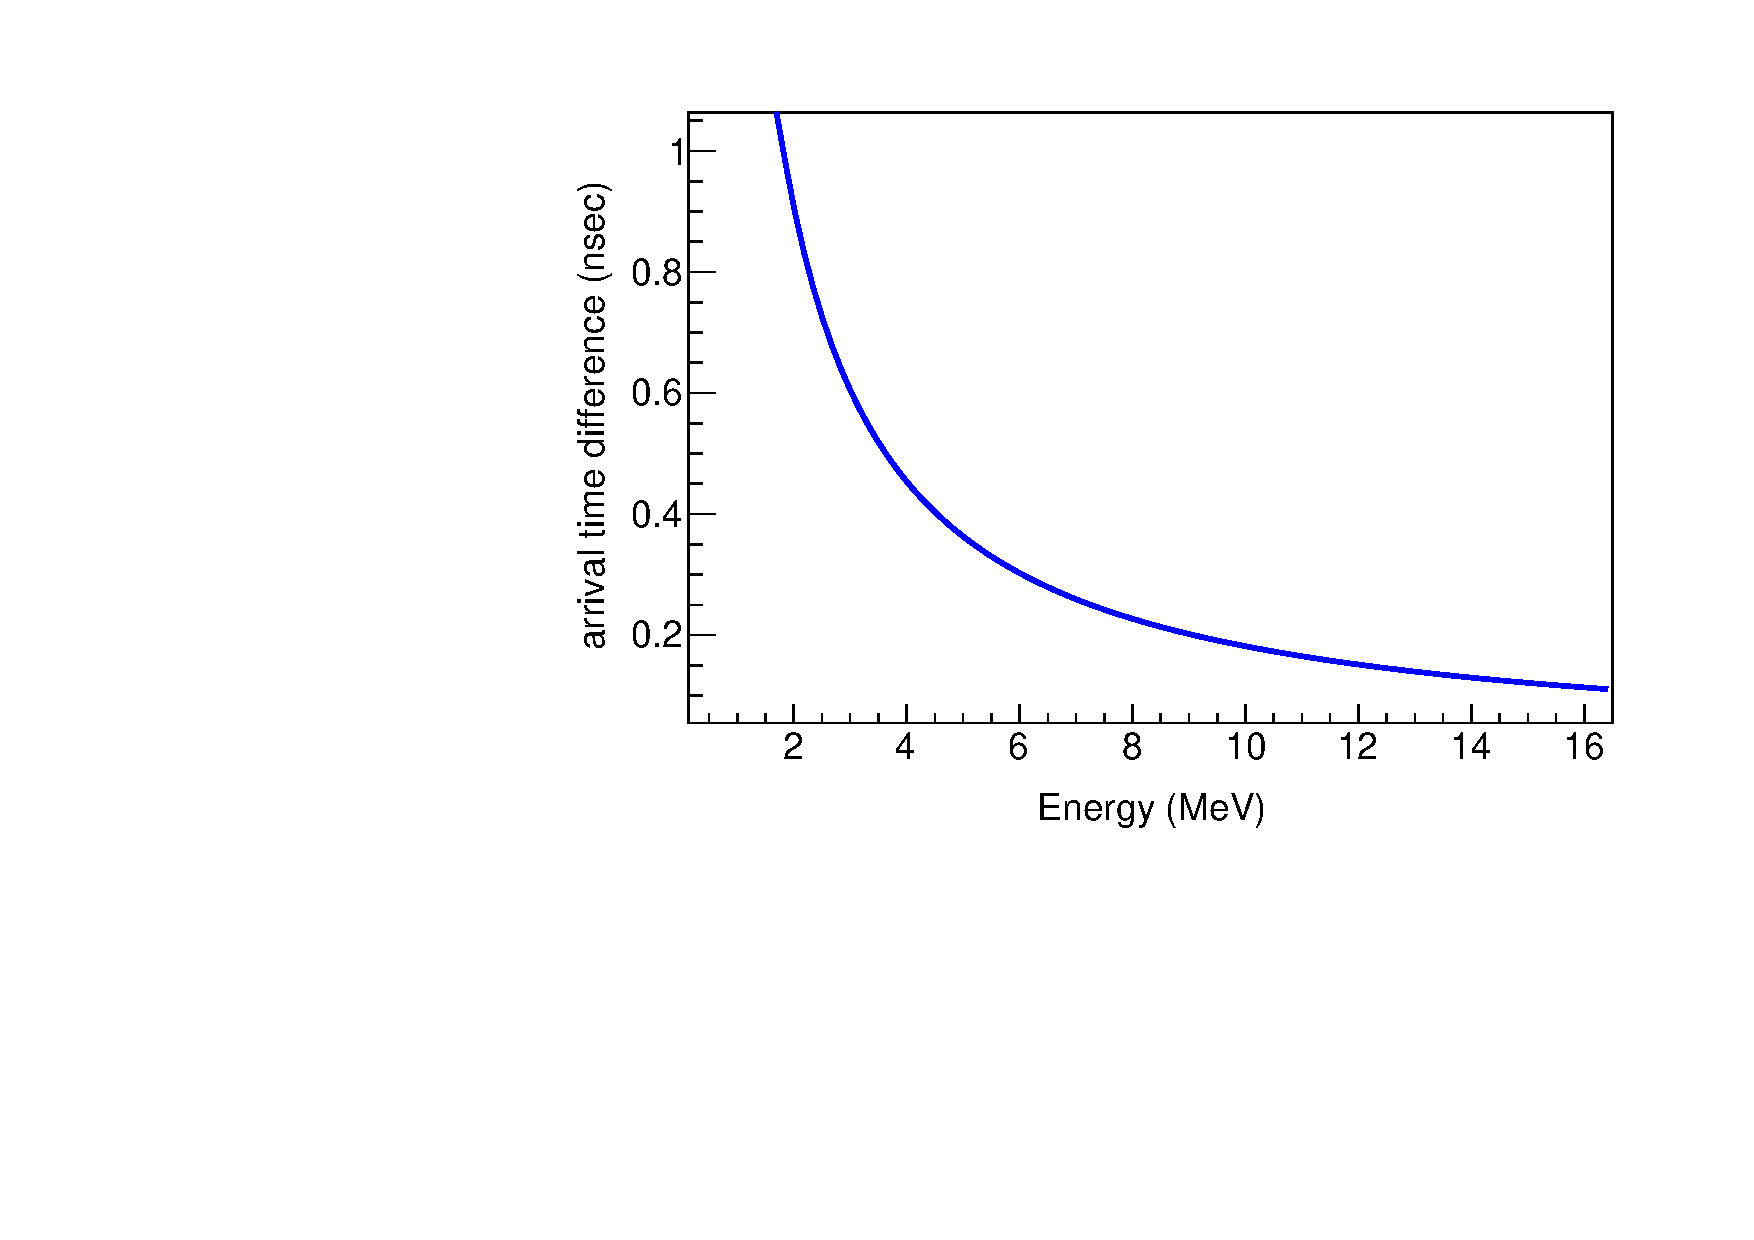
\includegraphics[width=0.5\linewidth]{Figures/deltaTvsE.pdf}} \\
 \includegraphics[width=0.49\linewidth]{Figures/parentEvsdT.pdf} &
 \includegraphics[width=0.49\linewidth]{Figures/nuEvsdT.pdf} \\
			\end{tabular}
%           	\begin{tabular}{c c}
%           	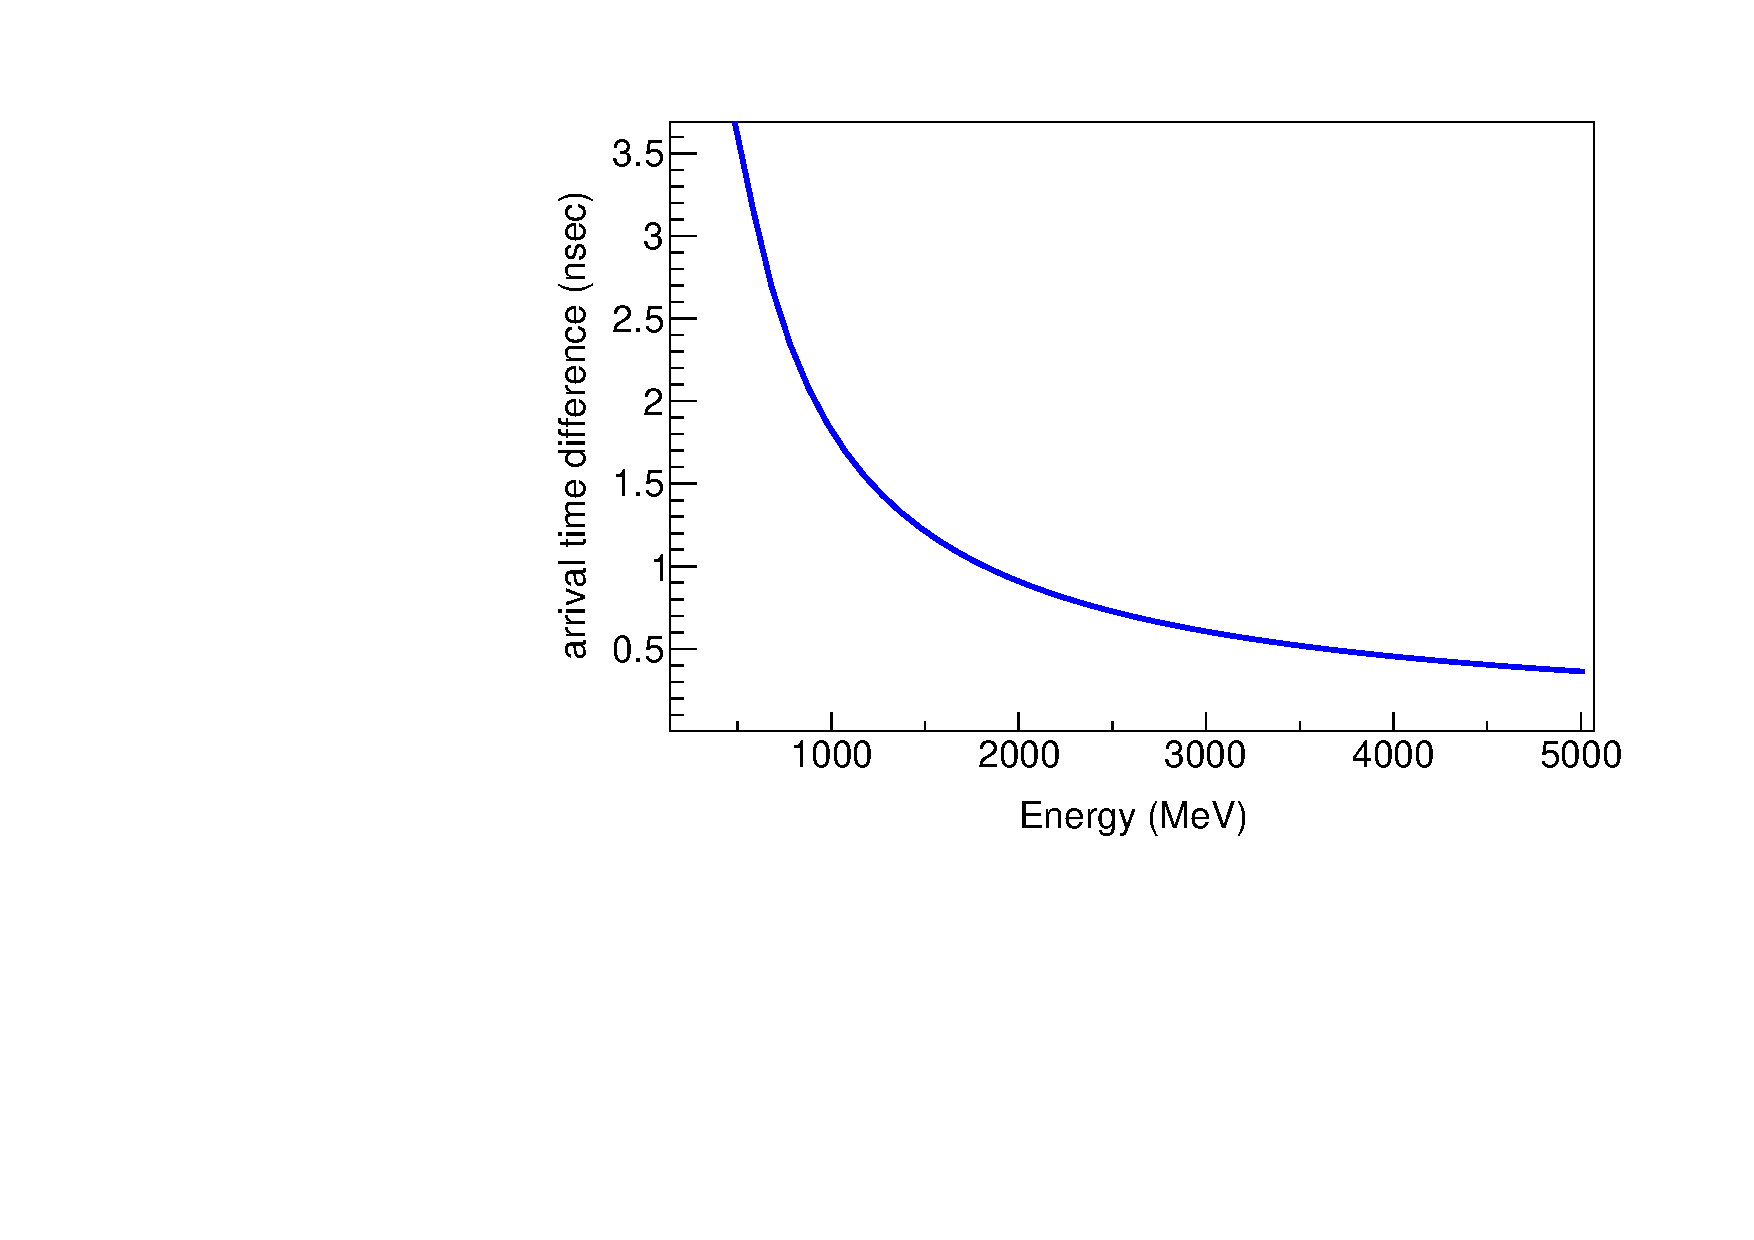
\includegraphics[width=0.455
%                  \linewidth]{Figures/2018.12.3_kinematics/deltaTvsE.pdf}
%                & \includegraphics[width=0.49
%                  \linewidth]{Figures/2018.10.14_LBNFtiming/parentEvsdT.pdf}
%                \\ \multicolumn{2}{c}{\includegraphics[width=0.5
%                    \linewidth]{Figures/2018.10.14_LBNFtiming/nuEvsdT.pdf}}
%			\end{tabular}
	\end{center}
	\caption{Top: A plot of the peak time difference between the arrival of neutrinos from a sub-relativistic pion of energy E' with respect to a relativistic pion (Eq~\ref{eq:beamkinematicsandtiming}). Bottom Left: The simulated relationship between the arrival times and pion energies, for a population of pions produced at the same time. Bottom Right: The equivalents plot of arrival time difference for different energies of the neutrinos.}
		\label{fig:beamkinematicsandtiming}
\end{figure}


\subsection{Impact of Bunch Size}
\label{bunch_size}

Just showing that wider bunches wash out the effect (short section)


%\begin{figure}[t]
%	\begin{center}
%           	\begin{tabular}{c c}	
%           	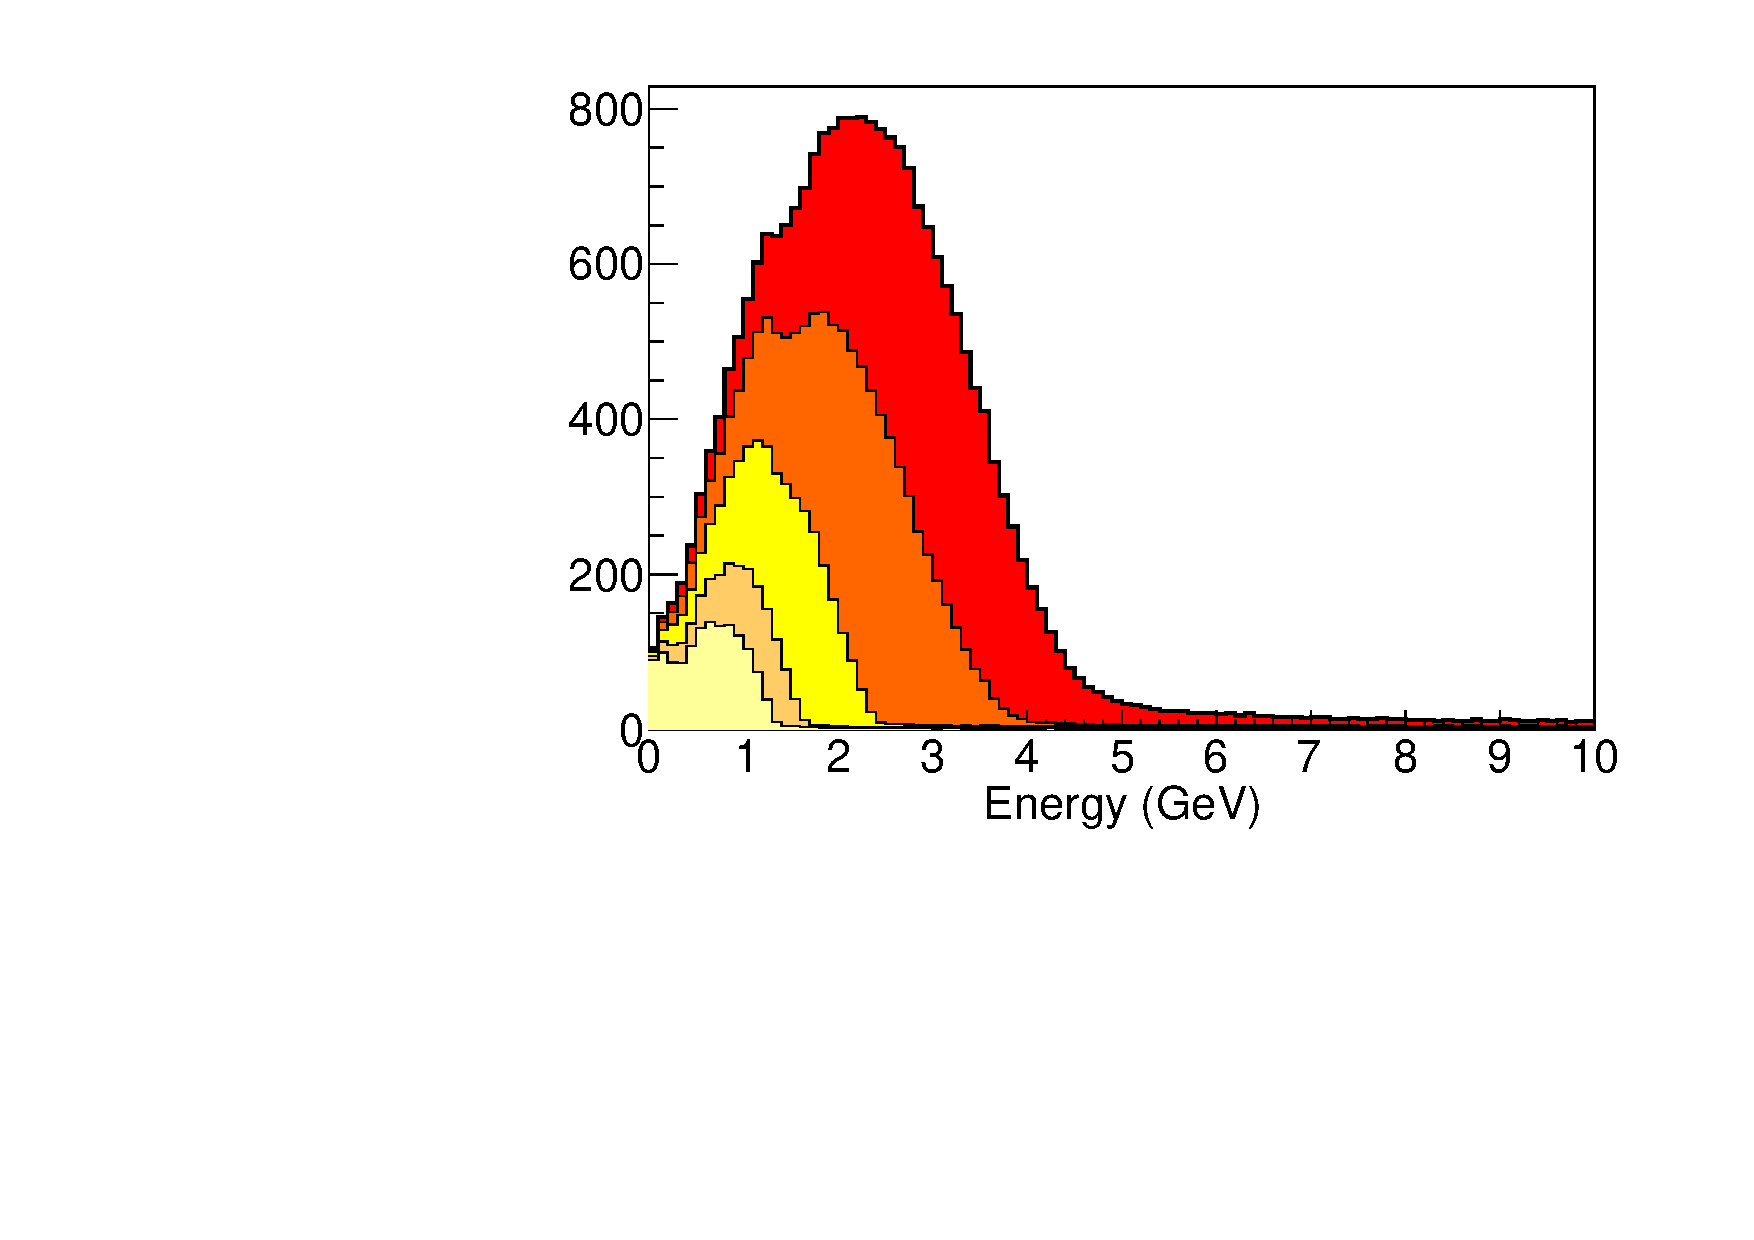
\includegraphics[width=0.49
%                  \linewidth]{Figures/DUNEbeam_truetimingB.pdf}
%                & 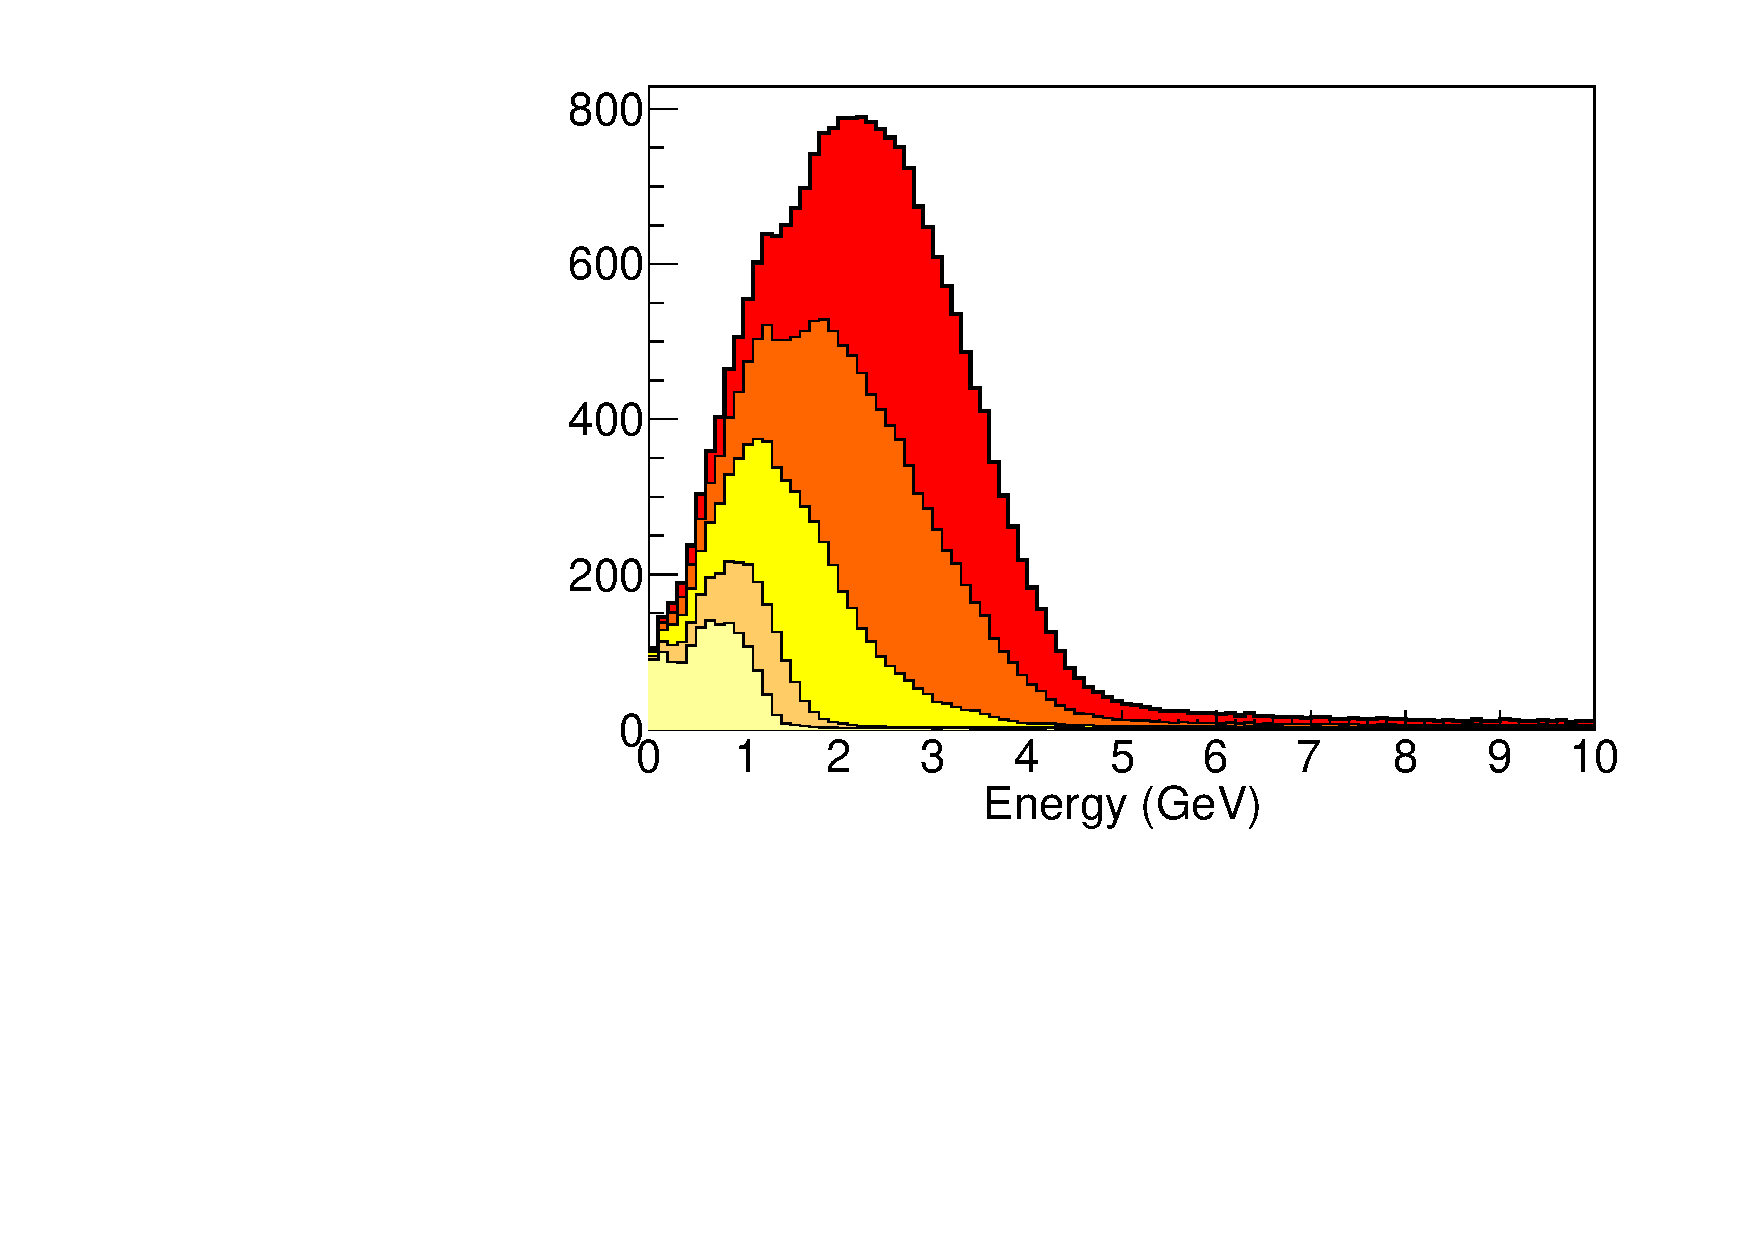
\includegraphics[width=0.49
%                  \linewidth]{Figures/DUNEbeam_100psecB.pdf}
%                \\ 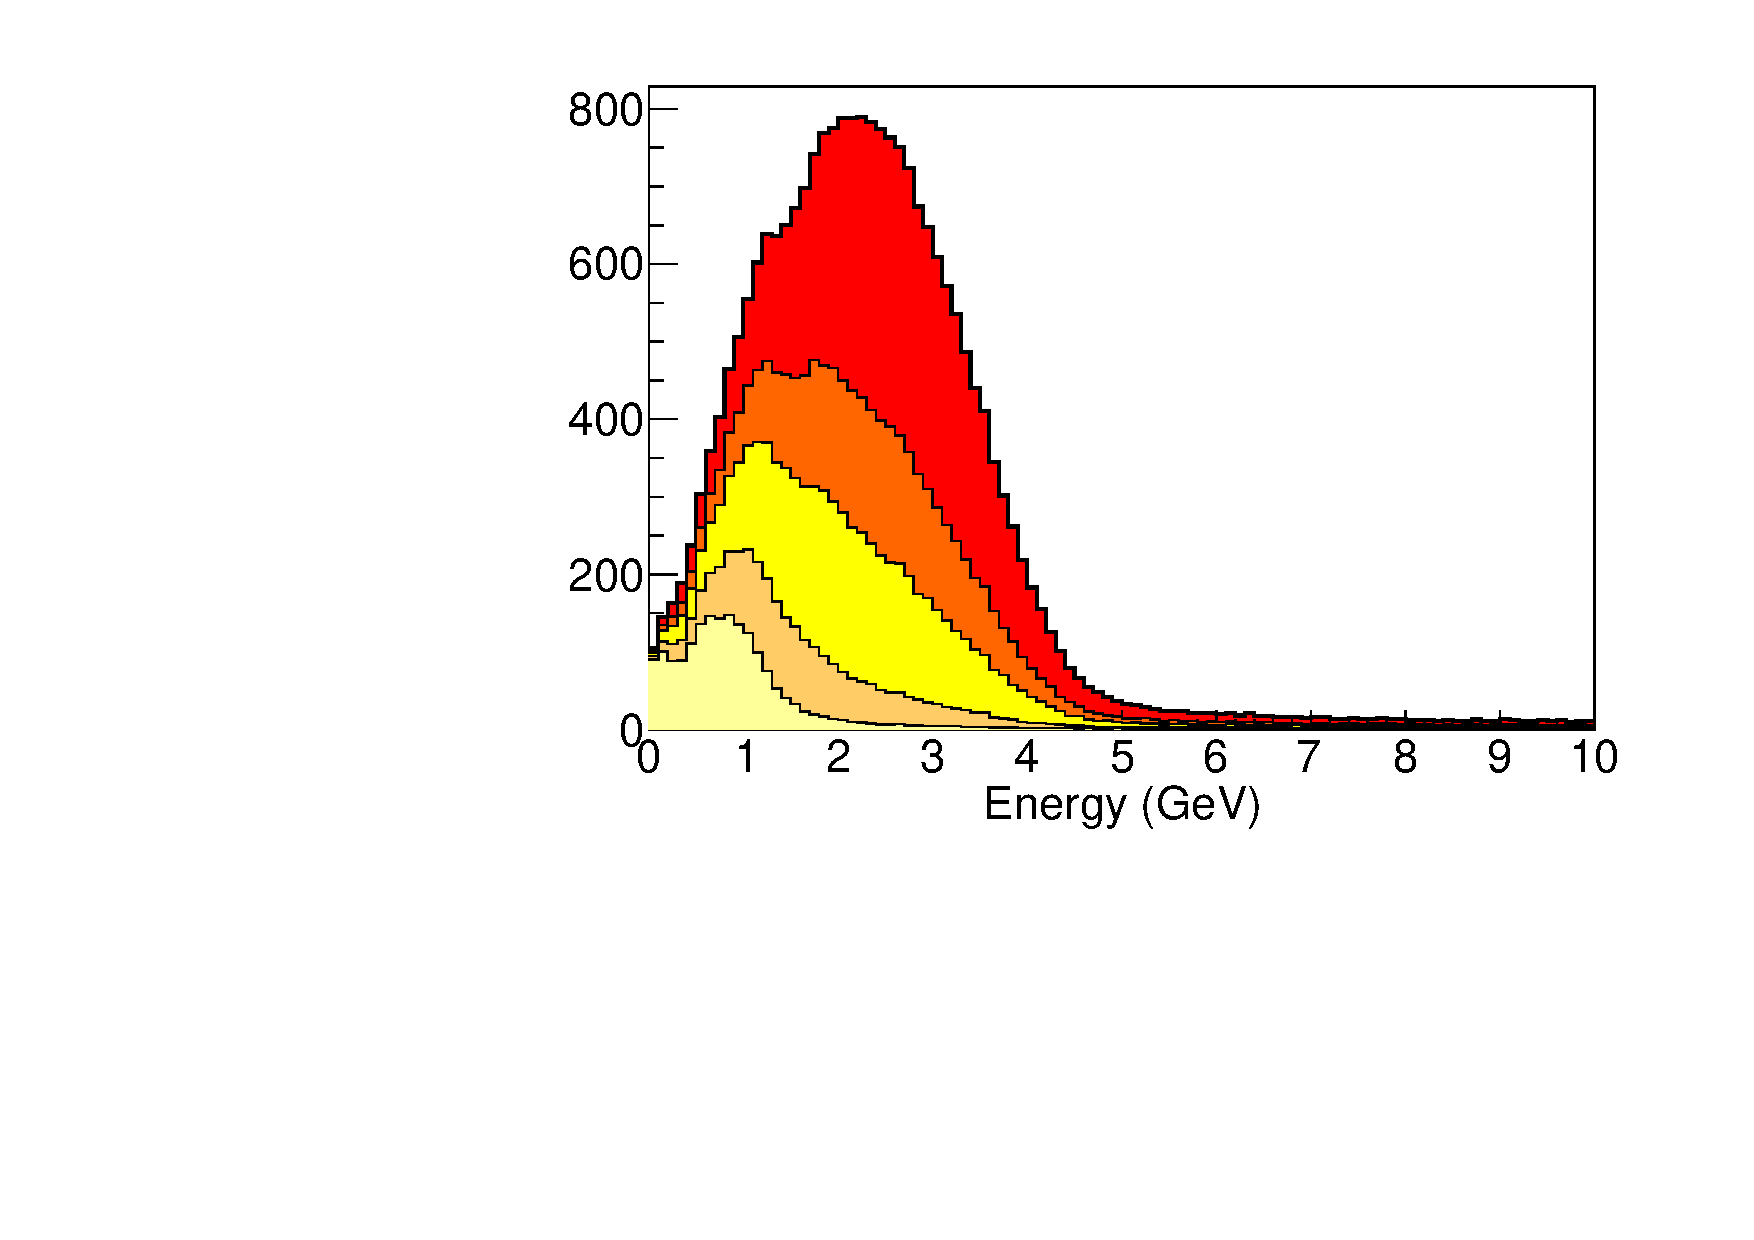
\includegraphics[width=0.49
%                  \linewidth]{Figures/DUNEbeam_250psecB.pdf}
%                & 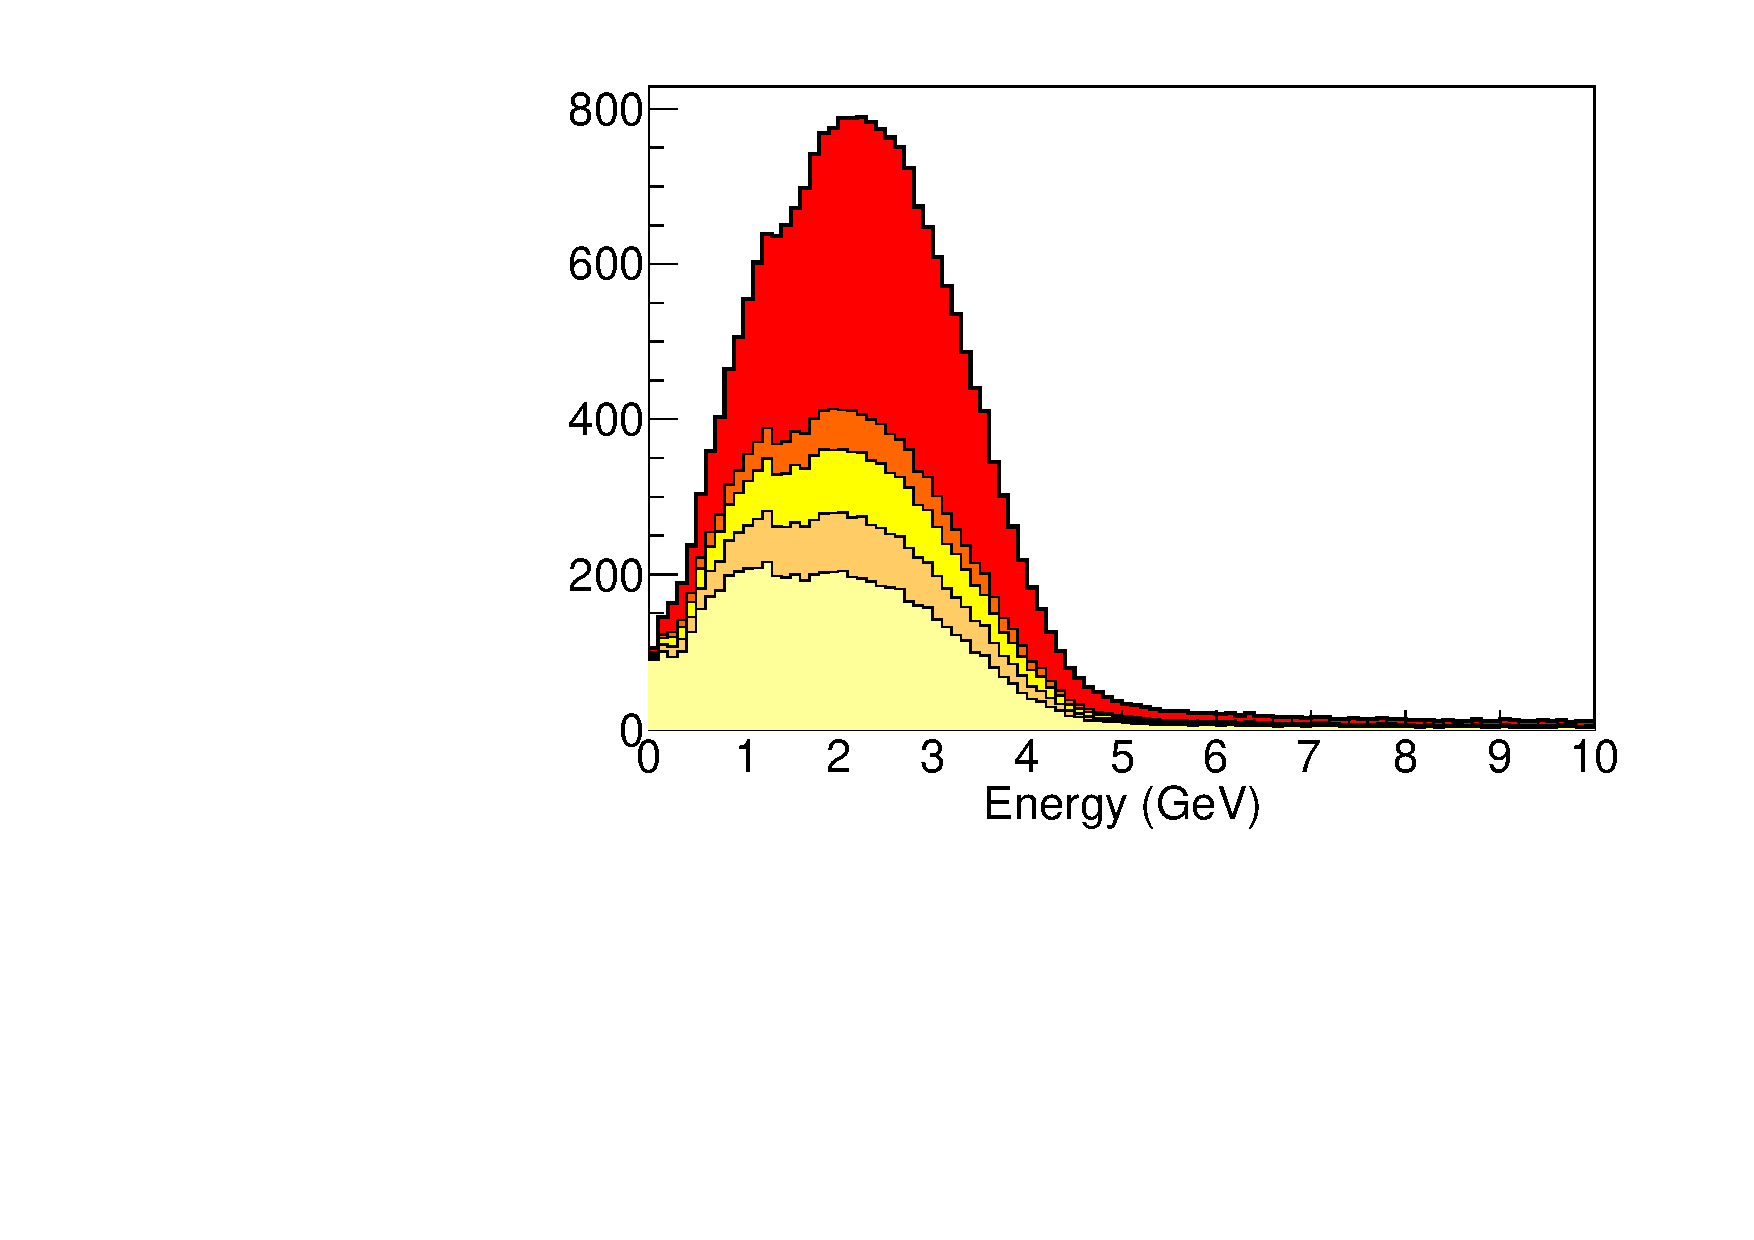
\includegraphics[width=0.49
%                  \linewidth]{Figures/DUNEbeam_900psecB.pdf}
%                \\
%			\end{tabular}
%	\end{center}
%	\caption{A series of panels showing the DUNE forward horn current flux (red), overlaid with the fluxes corresponding to increasingly later time-cuts on the bunch time, assuming no time spread of the protons on target: 250 psec after the start of the neutrino bunch (orange), 500 psec after (yellow), 750 psec (dark beige), 1 nsec (light beige). The UPPER LEFT panel corresponds to a case where all protons hit the target instantaneously. The UPPER RIGHT panel corresponds to a proton bunch with 100 psec width. The LOWER left panel corresponds to a 250 psec bunch width and the LOWER RIGT corresponds to 900 psec.}
%		\label{fig:anniedetector}
%\end{figure}


% End of Section 4


%%
% Section: Time-Sorted Energy and Flavor Spectra
%
\section{Time-Sorted Energy and Flavor Spectra}
\label{time_sorted_spectra}

Testing

\begin{figure}[ht]
	\begin{center}
           	\begin{tabular}{c c}
            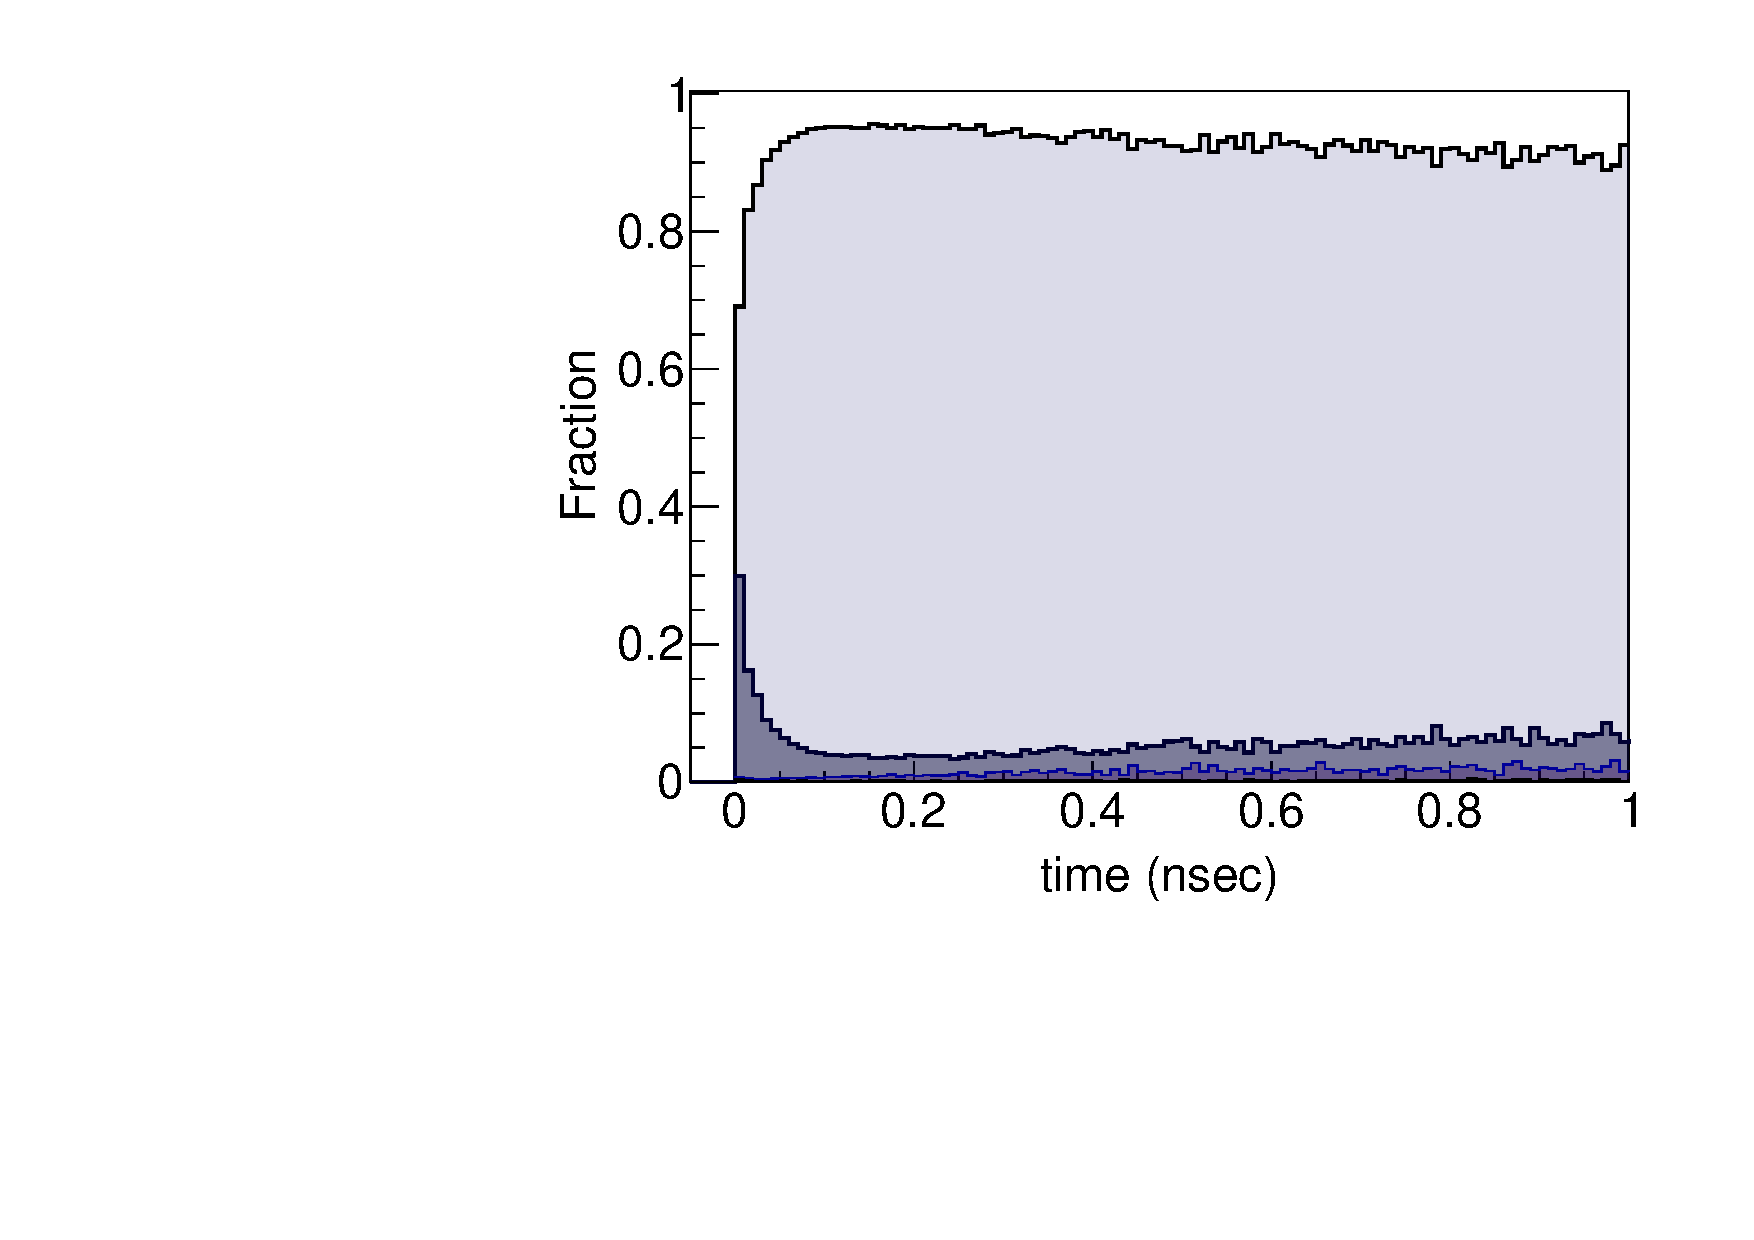
\includegraphics[width=0.48\linewidth]{Figures/NuFlava.pdf} &
            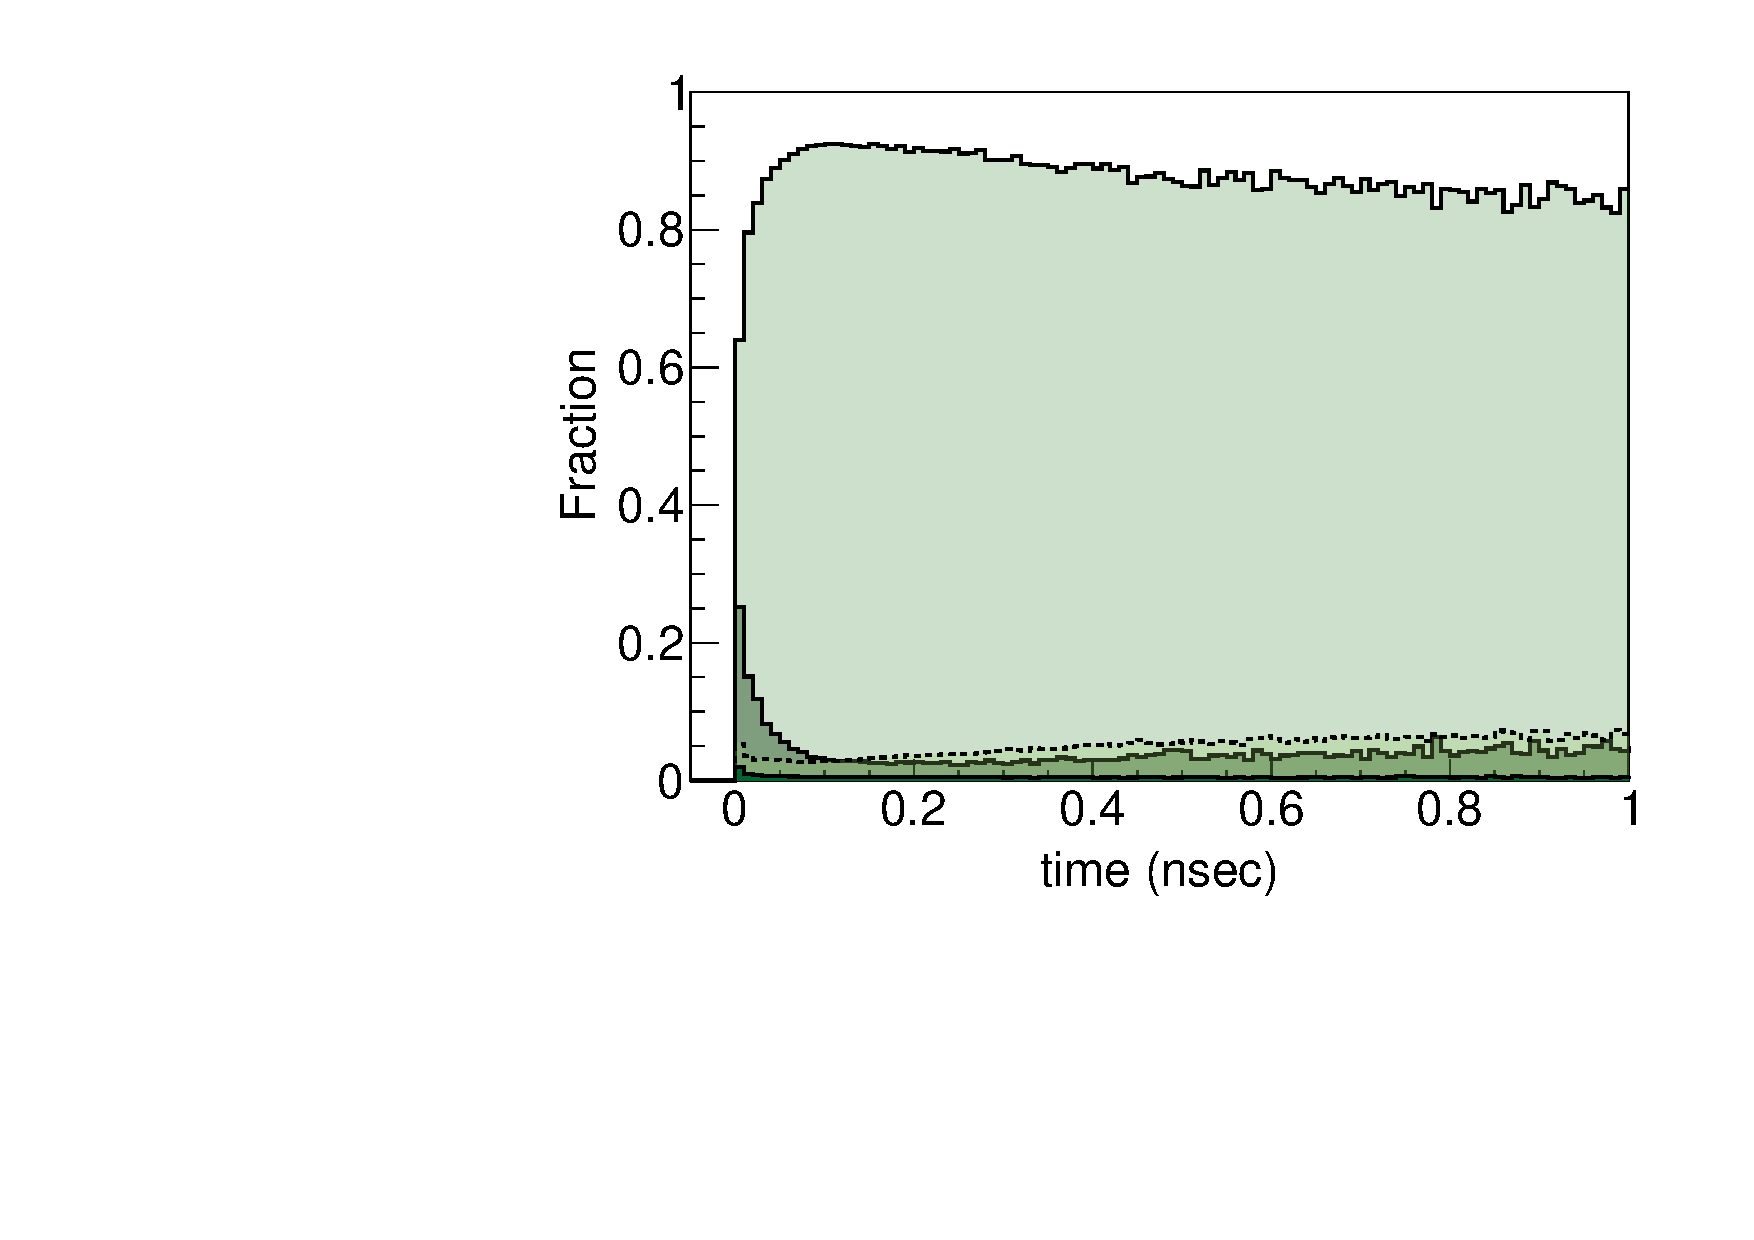
\includegraphics[width=0.48\linewidth]{Figures/NuParent.pdf} \\
			\end{tabular}
	\end{center}
	\caption{LEFT: The fractional composition of neutrino flavors in the beam as a function of time in Forward Horn Current (FHC): $\nu_{\mu}$ in light purple, $\bar{\nu_{\mu}}$ in light purple (wrong-sign contamination) in dark purlple, $\nu_{e}$ in red, and $\bar{\nu_{e}}$ in pink. RIGHT: The fractional composition of neutrino parents in the beam as a function of time: $\pi^{+}$ in dark green, $\pi^{-}$ in light green, K$^+$ in yellow, and K$^-$ in teal.}
	\label{fig:flavorandparentfrac}
\end{figure}


\subsection{Electron and Muon Neutrinos from $\pi$ and $K$ decay}
\label{mu_e}

\subsection{Tau Neutrinos}
\label{taus}

\subsection{Wrong Sign Contributions}
\label{wrong_sign}


%



\section{Accelerator Modifications: Rebunching protons at a higher RF frequency}
\label{RF}

The proton bunch must have as small a duration as possible in order to
select neutrino energies based on time of arrival at the
detector (see section \ref{mechanism}). This section describes one example of how to
create longitudinally thin proton bunches with time-widths on the order of 200 ps in the Fermilab Main Injector (MI) with minimal changes to the existing accelerating infrastructure. Outputs from a simulation of
this re-bunching scheme are presented.


\subsection{Properties of the present main injector proton bunch}
The main injector is filled with protons from the booster ring which
injects \textit{batches} of 8 GeV protons. Each batch contains 84 RF
\textit{buckets} at 53.1MHz. The MI has enough circumference to hold 7 batches, or 588 buckets, but is only filled with 6 batches leaving an \textit{abort gap} of 84 buckets for the \textit{kicker} which directs the
 beam into the NuMI target. Every 1.2 s (referred to below as the \textit{cycle
  time}), the kicker is engaged and 6 batches of protons are extracted
into the NuMI target downstream, creating about 10 $\mu$s of bunched
neutrino beam.

The longitudinal position of a proton in the bunch changes depending
on its momentum. Each proton in the bunch occupies a point in the
phase space of RF phase $\phi$ (or longitudinal location in the bunch)
and momentum relative to the synchronous particle momentum, $\delta =
\mathrm{d}p/p_0$. A particle with $\delta = 0$ will not change phase in the bunch over time. 

Each main injector RF bucket is about 20 ns long but the protons occupy a small 
fraction of the bucket. Protons from the booster enter the main injector with a
$(\phi, \delta)$ phase-space area of about 0.2 eVs (95\% of particles). Each MI bunch
is a combination of two slip-stacked booster bunches, which after acceleration leads to
about 0.7 to 1 eVs of phase space area. This proton bunch is
non-gaussian with an RMS time-width of about 900 ps (cite). At 1 eVs, this implies that 

\begin{equation}
\mathrm{d}p_{rms} = \frac{A}{6\pi t_{rms}} \simeq \frac{1 [\texttt{eVs}]}{6\pi\times 1 [\texttt{ns}]}  \simeq 53 \quad \texttt{MeV}
\end{equation}

or a $\delta$ of $4.4\times 10^{-4}$. An attempt to generate this initial particle distribution
is used in the simulations below and is shown in red in figure \ref{fig:bunch_distributions}.


\subsection{Higher frequency RF structure and hardware}

The main injector proton bunch will need to be re-bunched into a
roughly 10-times higher frequency RF structure in order to achieve a
goal of 100 - 200 ps bunch width for doing stroboscopic neutrino physics. An
insertion of only one such RF cavity into the existing ring would
allow for higher frequency re-bunching.

The company \textit{Research Instruments} commercially produces
superconducting RF cavities at 500MHz for use in electron storage
rings like the Canadian Light Source
\cite{nsls-cavity}\cite{cls_stampe}\cite{research_instruments}. These
cavities are designed to operate at 2 MV RF amplitude which is within the
voltage amplitudes supplied to the present main injector cavities.
 The commercial availability of such cavities is encouraging,
as this cavity could be used in prototyping and early testing of the
re-bunching sequence. 


\subsection{Example of a rebunching procedure in the Fermilab Main Injector}

A simulation has been written to study the following properties of a
rebunching procedure: the ramp-down/ramp-up functions for re-bunching
at a higher frequency, the final RMS bunch width, and the total
additional time needed to re-bunch. These quantities will place
constraints on the re-bunching cavity as well as shed light on the
impact to neutrino physics for a given loss in total POT.

\subsubsection{Simulation equations}

The simulation presented uses the self-consistent beam
longitudinal synchrotron motion in a circular accelerator:

\begin{equation}
\dot{\delta} = \frac{\omega_0 e V_{rf}}{\beta ^2 W}\sin(\phi) 
\end{equation}
\begin{equation}
\dot{\phi} = -2\pi h \eta \delta \omega_0
\end{equation}

where $\omega_0$ is the RF cavity frequency ($\phi = \omega_0 t$),
$\delta$ is the $\mathrm{d}p/p_0$ momentum fraction relative to the
synchronous reference momentum $p_0$, $V(\phi) = V_{rf}\sin(\phi)$ is
the RF voltage function with amplitude $V_{rf}$, $\beta$ is the
relativistic velocity of the protons, $W = E + m_p$ where $m_p$ is the
mass of the proton and $E$ is the design energy of the beam, $h$ is
the harmonic number, and $\eta$ is the phase slip factor.

A first order discrete approximation of these equations can be used to
calculate particle dynamics in $(\phi, \delta)$ phase-space

\begin{equation}
\delta_{n+1} = \delta_n +  \frac{e V_{rf}}{\beta ^2 W}\sin(\phi_n) 
\end{equation}
\begin{equation}
\phi_{n+1} = \phi_n - 2\pi h \eta \delta_{n+1} 
\end{equation}

For two RF voltage functions with frequencies $f_{1}$ and $f_{2}$
superposed, the first equation becomes

\begin{equation}
\delta_{n+1} = \delta_n +  \frac{1}{\beta ^2 W}(eV_{1}\sin(\phi_n) + eV_{2}\sin(\frac{f_2}{f_1}\phi_n)) 
\end{equation}

\subsubsection{Voltage transition functions}

In a study of beam preparation for the Fermilab g-2 experiment,
K.Y. Ng explores functions for adiabatic voltage changes of cavities
that preserve area in longitudinal
phase-space. \cite{adiabatic_capture}. One function that follows from
the adiabatic condition $\omega_s \gg \frac{1}{A} \frac{\mathrm{d}
  A}{\mathrm{d}t}$ is

\begin{equation}
V(t) = \frac{V_0}{[1 - (1 - \sqrt{V_0/V_1})t/t_1]^2}
\end{equation}

for ramping voltages up ($V_1 > V_0$), and 

\begin{equation}
V(t) = \frac{V_0}{[1 + (\sqrt{V_0/V_1} - 1)t/t_1]^2}
\end{equation}

for ramping voltages down. These functions will be referred to as
\textit{adiabatic} voltage functions.

An example of a re-bunching recipe is shown in figure
\ref{fig:transition_voltages}. The end point voltage of 2 MV for the
higher frequency cavity is set by the specifications of the cavities
available from Research Instruments. The starting voltage of 2 MV for
the 53.1 MHz structure is set by the operating parameters of the
Fermilab main injector. Timescales of around 60 ms total will be
needed to preserve 95\% of the POT for neutrino experiments, as the design cycle time is 1.2 seconds.


\begin{figure}[h!]
	\begin{center}
        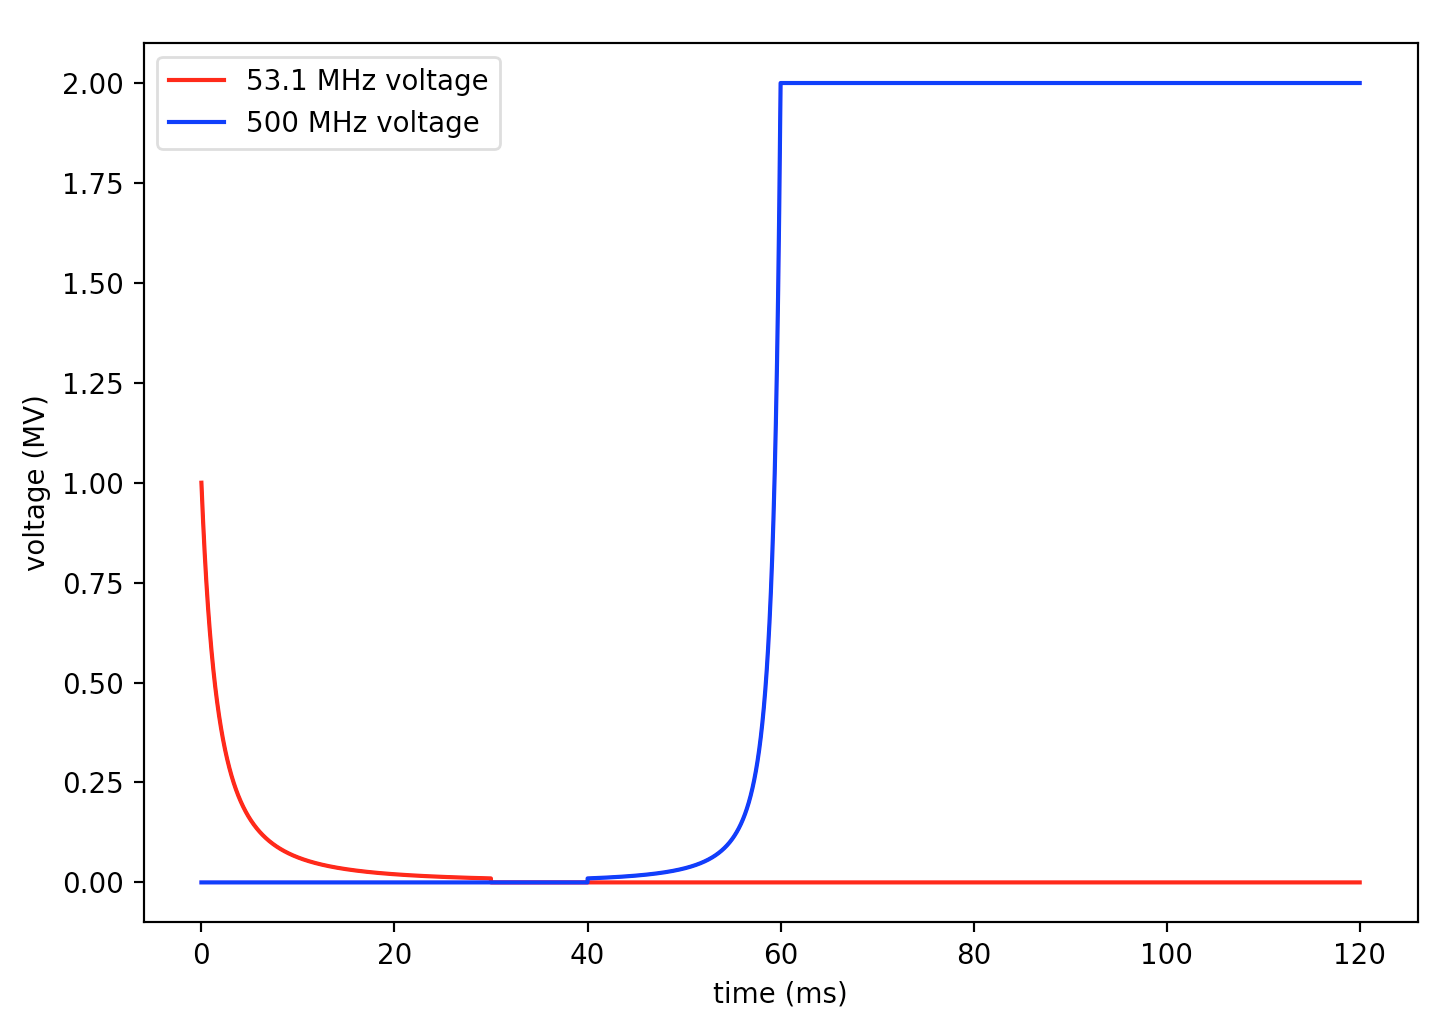
\includegraphics[width=0.60\linewidth]{Figures/transition_voltages.png}
	\end{center}
	\caption{An example of the applied voltages to the 53.1 MHz
          cavities (red) and the 500 MHz cavity (blue). Both are adiabatic voltage
          ramp-up/ramp-down functions, where the 53.1 MHz cavities start at 1MV and
          the 500 MHz cavities end at 2MV. Both cavities in the simulation have a minimum
          voltage of 10 kV. In this example, there is 10 ms of time after the ramp-down has
          ended and the ramp-up of the 500 MHz cavity begins.}
		\label{fig:transition_voltages}
\end{figure}

\subsubsection{Results of one recipe for re-bunching}

\begin{table}[h!]
\begin{tabular}{|p{0.3\textwidth}|p{0.3\textwidth}|p{0.4\textwidth}|}\hline
\textbf{Parameter} & \textbf{Value} & \textbf{Note} \\ \hline
Beam particle mass & 938 MeV  & protons \\ \hline
Synchronous momentum & 120 GeV & \\ \hline
Transition gamma $\gamma _t$ & 20.4 & \\ \hline
Harmonic number & 588 & 84 bucketes and 7 batches\\ \hline
Number of simulated particles & $2\times10^5$ & \\ \hline
Initial proton bunch $\delta$ & $3\times10^{-4}$ gaussian std & \\ \hline
Initial proton bunch phase & 870ps with 2 ns halo gaussian stds & halo is 5\% of central particles \\ \hline \hline
RF frequencies of cavities & 53.1 MHz and 500 MHz & 500 MHz used to match commercial cavity \\ \hline
$V_0 ^{53}$ and $V_1 ^{53}$ & 1 MV and 10 kV & Voltages for adiabatic function, set to 0 V at endpoint \\ \hline
$V_0 ^{500}$ and $V_1 ^{500}$ & 10 kV and 2 MV & Voltages for adiabatic function, set to 0 V at endpoint \\ \hline
Time between voltage ramps & 10 ms & where both RF voltages are 0 V \\ \hline
Resulting 1/e RF bucket egress into abort gap & XXX buckets & on either first bucket or last bucket \\ \hline
\end{tabular}
\caption{Parameters used in the simulation of synchrotron motion for re-bunching.}\label{tab:accsim_parameters}
\end{table}

Phase space distributions at various times are shown in figure
\ref{fig:bunch_distributions} for a simulation that takes the voltages
from figure \ref{fig:transition_voltages} as an input. The red
particles represent a best estimate of the present design proton
distribution in the main injector before extraction. 

Projections of the initial and final phase space variables
are shown in figure \ref{fig:bunch_projections}. 

\begin{figure}[h!]
	\begin{center}
        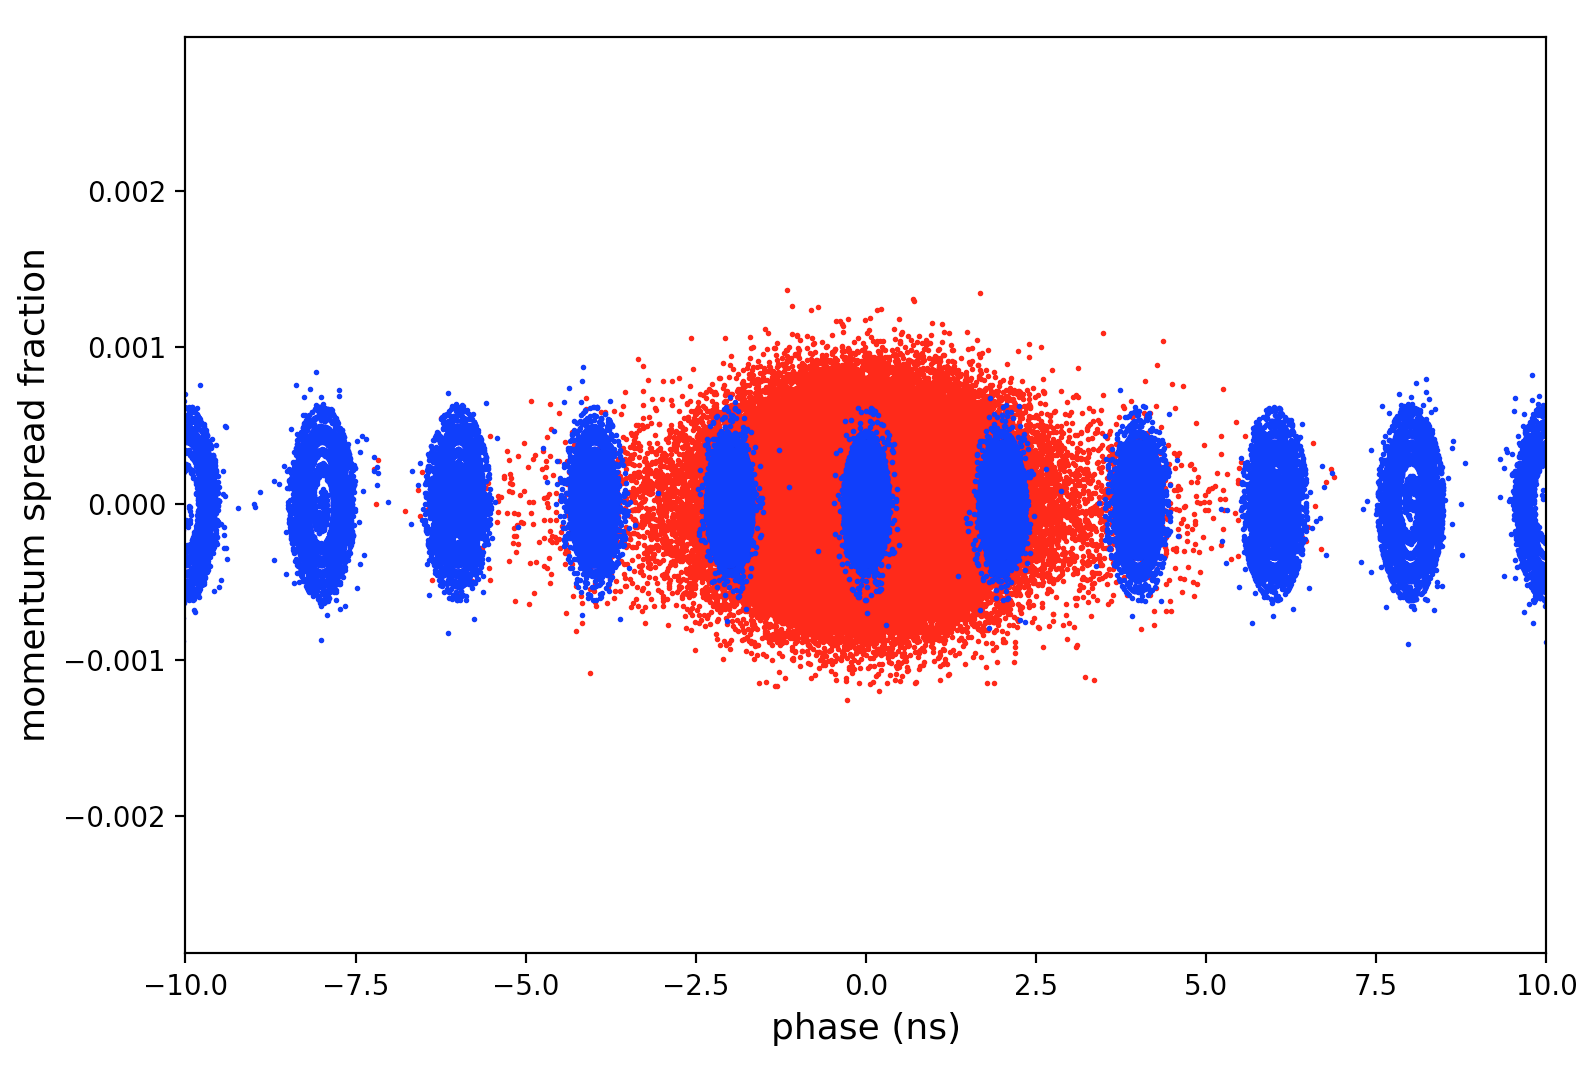
\includegraphics[width=0.60\linewidth]{Figures/bunch_distributions.png}
	\end{center}
	\caption{Distribution of protons in energy spread vs. RF phase
          for the initial main injector proton bunch (red), the
          transition time between the two RF frequencies (green), and
          the end point after ramping the high frequency voltage
          (pink). This particular rebunching took a total of 50ms, a
          4\% addition to the total cycle time.}
		\label{fig:bunch_distributions}
\end{figure}

\begin{figure}[h!]
	\begin{center}
        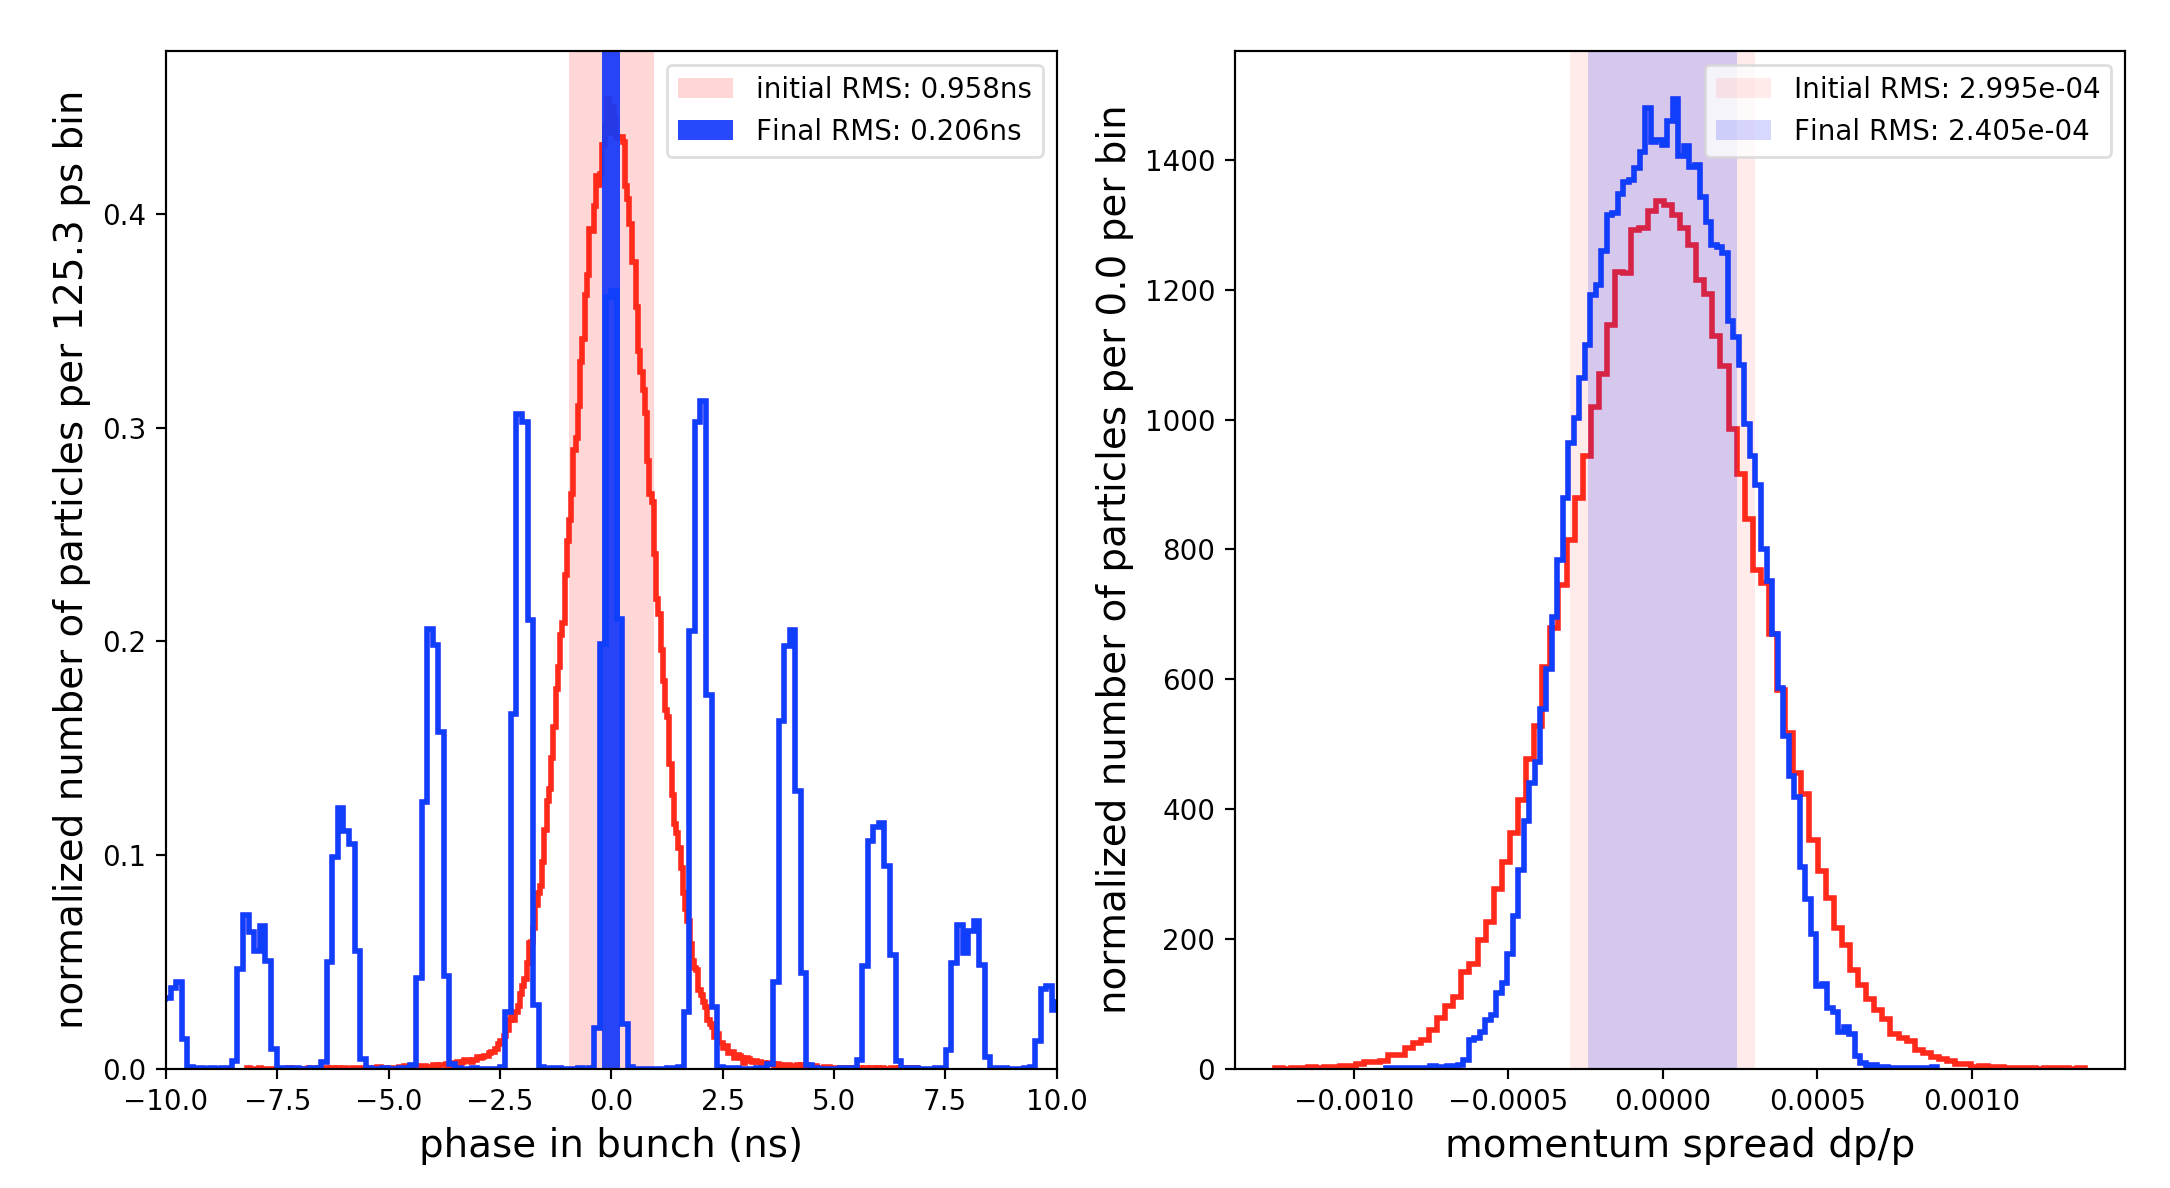
\includegraphics[width=0.60\linewidth]{Figures/bunch_projections.png}
	\end{center}
	\caption{Projection of the initial and final bunches onto the phase space variables $\phi$ and $\delta$. 
	The final longitudinal position of particles extends out past the initial RF bucket window, and these
	particles will be captured into neighboring RF buckets. The end-point buckets will leak particles into 
	the abort gap for the kicker. 95\% of the particles will be contained within the first *** buckets of the abort gap on either side (see table \ref{tab:accsim_parameters})}
		\label{fig:bunch_projections}
\end{figure}

The objective of the rampdown of the 53.1 MHz voltage amplitude is to
create a thin line in $(\phi, \delta)$ phase-space. A thinner
distribution before applying higher frequency cavity voltage will lead
to smaller time-width bunches after the higher frequency cavity
voltage reaches 2 MV (cite Evan's technical write-up). The momentum spread at the transition
time is largely dictated by the ramp-down functions and their time
parameters. Therefore, the thin-bunch time-width RMS was explored as a
function of total re-bunching time where the ramp-down time is varied.

Figure \ref{fig:bunch_width_curve} plots the final RMS time-width as a
function of the total re-bunch time divided by the main injector cycle
time. The fraction on the x-axis is equal to the loss in POT from
time-on-target alone.

\begin{figure}[h!]
	\begin{center}
        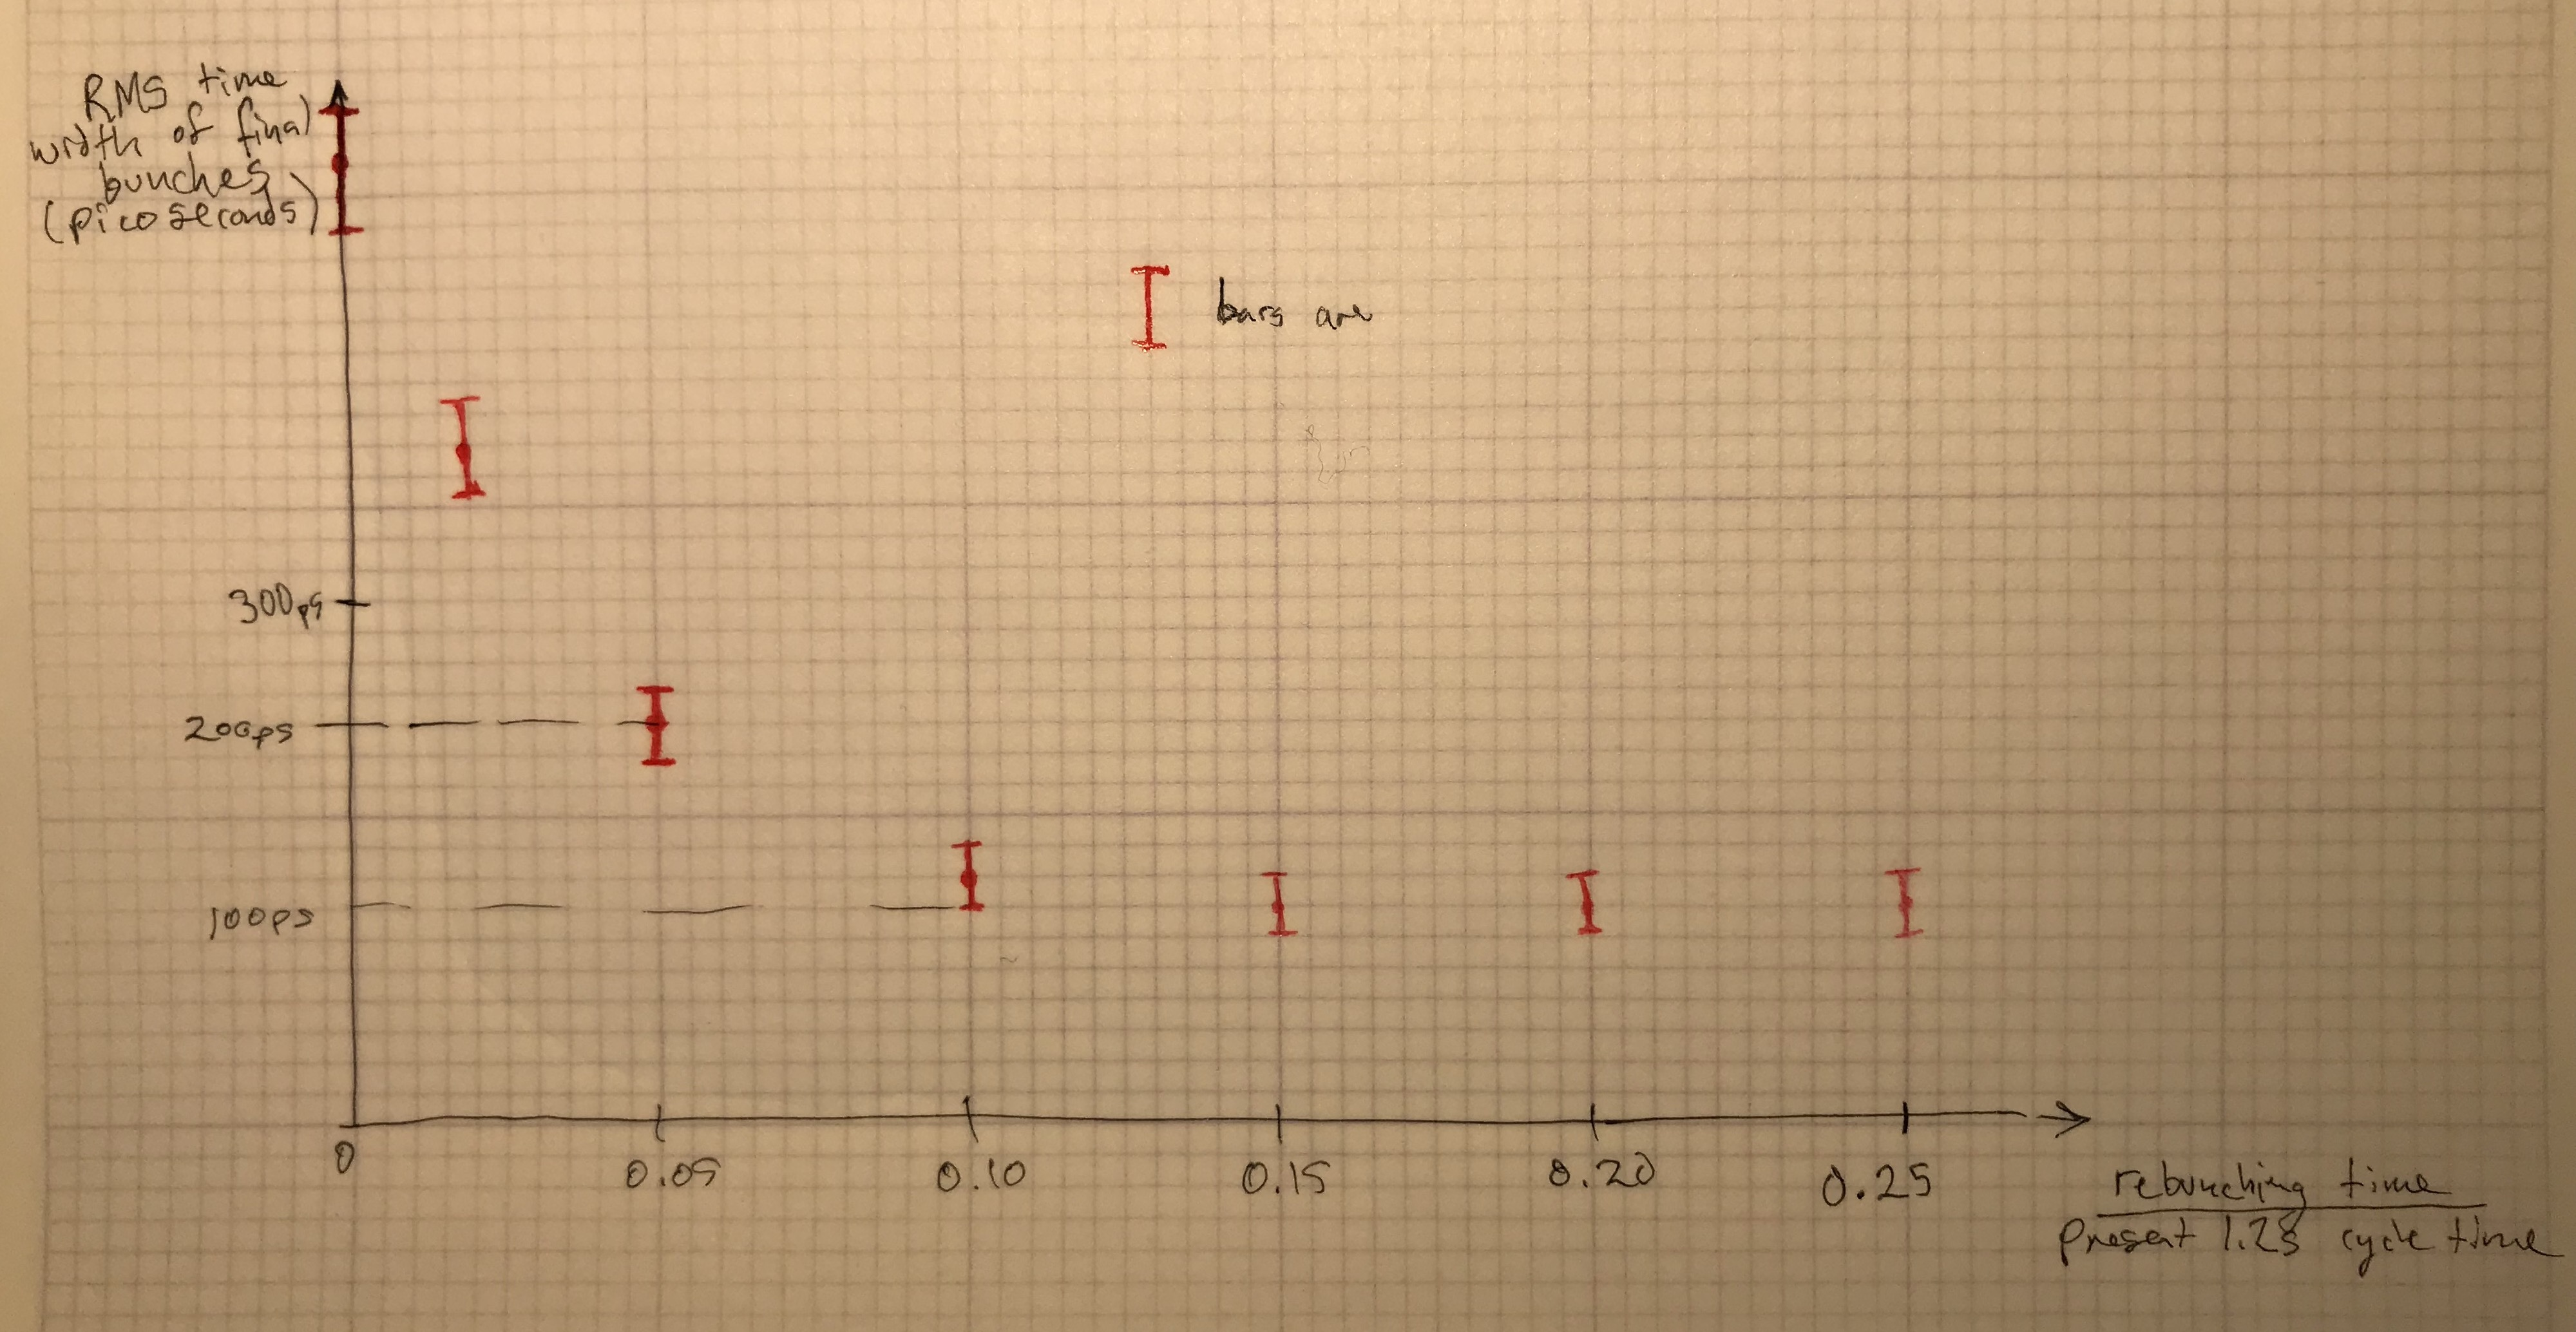
\includegraphics[width=0.60\linewidth]{Figures/draft_rms_vs_time.JPG}
	\end{center}
	\caption{The average thin-bunch time-width root-mean-square after going through a
          re-bunching procedure that takes time $t$, where the x-axis
          is the ratio of $t$ to the present cycle time of $1.2$
          seconds. Longer re-bunching time corresponds to a reduction
          in POT because it increases the period between main injector
          dumps.}
		\label{fig:bunch_width_curve}
\end{figure}

This simulation shows that bunch widths on the order of 200 ps may be
achieved given a single RF cavity at about 500 MHz and the properly
optimized voltage functions for re-bunching without too much more than
5\% loss in POT.

% End of Section 6


%
% Section Muon Monitor
%
\section{Using Muons and Fast Photodetectors to Measure the Bunch-by-bunch Proton Intensity Profiles}
\label{muon_monitor}

The stroboscopic technique relies on the precise time relationship
between a given proton parent bunch interacting in the target and the `grandchild' neutrino
events detected in the neutrino detectors. We propose using fast
photodetectors to measure the intensity profile of the proton
interactions on a bunch-by-bunch basis with a resolution sufficient to
allow `time-slicing' of the neutrino vertices in the detector for
energy and flavor discrimination. For example, 10 psec resolution
on the profile of each proton bunch would introduce little smearing in 100 psec
time-slices at the neutrino detector.

%\subsection{Muon Monitor Systems}

The monitoring would be done with two conventional muon monitor
systems, one at 90 degrees to the target in the Lab frame (the
Transverse Muon Monitor System, or TMMS), and one
embedded in the shielding at the end of the decay volume (the Forward
Muon Monitor System, or FMMS). Each would
consist of photodetectors and waveform sampling electronics capable of a
time resolution on the order of 10 psec.


%\subsubsection{Transverse Muon Monitor System (TMMS)}
The transverse muon monitor system (TMMS) provides a bunch-by-bunch
profile of the proton interactions in the target. The TMMS consists of
a small area MCP-PMT Cherenkov telescope located on a vertical line to
the target, with substantial shielding between the target and the
counters. The telescope could be located above ground, or, as was done
in Ref.~\cite{E100}, located in a cladded hole drilled into the
ground, as determined by the rate and the desired momentum cut-off
provided by the muon range in the transverse shielding.

The TMMS views the proton bunches transversely, so that the time
offsets in the longitudinal direction do not introduce biases in the
proton bunch profile from energy-dependent effects. The flight path in
the transverse direction can be made to be short. The smearing in time of
hadron decay, even though independent of the longitudinal bunch
profile, would wash out the bunch structure. In addition to the short
decay path, the shielding in the
transverse direction will provide a lower momentum cutoff for muons, and
hence for parent hadrons, being determined by the minimum muon range
required to reach the TMMS.

%\subsubsection{Forward Muon Monitor System (FMMS)}
The forward muon monitor system (FMMS) provides a
bunch-by-bunch profile of muon neutrino production in the target. The
TMMS would consist of a large-area `range stack' of large-area MCP-PMT
photodetectors with precise time resolution, separated by shielding so
as to measure the energy spectrum of the muons by range. In addition,
each layer would consist of multiple \LAPPDTM modules in a transverse
pattern capable of measuring the directional information as well
as the time profile of the proton beam.

The FMMS directly records the muon time of arrivals in each
layer. The muon times are determined by the flight time of the parent
hadrons in the same way as the neutrino times measured at the
detector. As the mix of electron and muon neutrinos is energy and sign
dependent, the FMMS provides additional family information as well as
a stroboscopic measurement of the muon spectrum.

%\subsection{Photodetectors, Waveform Sampling, and Data Acquisition}

%
% Section: Synchronization of the Bunch Profile with the Neutrino
% Interaction Time
% 
%\subsection{Synchronization of the Bunch Profile with the Neutrino Interaction Time}
%\label{synchronization}
%\subsection{Time Stamps and Latency Budgets}
%\subsection{Local Clocks}
%\subsection{Synchronization of Local Clocks}
%\subsection{Monitoring and Verification}
The neutrinos arrive at both the near and far detectors before any
electronics signal can propagate, creating a substantial latency
between the proton bunch profile and the corresponding neutrino event profile.
Consequently at both the target and the detector there needs to be a
wave-form sampling and digital buffer with enough bandwidth to keep up
with the RF bunch frequency and enough depth to allow for the latency,
triggering, and readout. 

Several standard schemes employed at high
luminosity colliders and waveform sampling systems would mitigate high
data rates. Local processing in FPGAs located in the front-end
electronics allows sparcification and data compaction. Multiple buffering will allow deadtimeless
operation.  FPGAs also allow prescaling, with a small fraction of
bunches outputting the full sampling profile, with the bulk only
transmitting as many fitted moments as prove necessary to monitor
shapes over the time scale set by the prescale.

The synchronization of the neutrino event with its parent proton bunch
consequently is done with time stamps in both locations. This requires
a master clock available to both locations. One solution is two
synchronized atomic clocks, which have the requisite
accuracy~\cite{atomic_clocks}. 

Monitoring and verification of the synchronization is
necessary~\cite{speedy_italians}. Accumulated data at the `edges' of the
proton bunch train may verify that events only occur in occupied
bunches, registered to the correct timing.




% Section Detection Feasibility
%
\section{Achieving Sub-Nanosecond Time Stamping of Neutrino Interactions}
\label{Detection Feasibility}

\subsection{Beam Monitoring}

\subsection{Near Detector Considerations}

\subsection{Far Detector Considerations}

\subsubsection{Vertex Resolution}

\subsubsection{Global Time Stamping}

% End of Section 7



%
% Section Results
%
\section{Results}
\label{results}
Results...
\subsection{Delta-Function Proton Bunch}
Plots go here and in each subsequent subsection
\subsection{Comparisons of 53 MHz and  500 MHz RF Structures}
More plots
\subsubsection{Forward Horn Configuration}
More plots
\subsubsection{Reverse Horn Configuration}
More plots
\subsubsection{Tau Neutrinos}
More plots
\subsection{Near vs Far Detector Considerations}
More plots

% End of Section 7



%
% Section Conclusions
%
\section{Conclusions}
\label{conclusions}
A higher RF frequency than the current 53 MHz RF structure in the
Fermilab Main Injector (MI) would allow using precision time
measurements to statistically discriminate the energy and family of
neutrino events in on-axis detectors. For narrow proton bunches, the
time of the neutrino interaction in the near or far neutrino detector
relative to the production of the parent hadron in the target is
weighted towards lower energy for later events and higher energy for
earlier events. Selecting on time bins (a.k.a. the `stroboscopic'
technique) relative to the RF thus performs a similar sculpting of the spectrum for an on-axis geometry as going off-axis without losing the on-axis flux. The relative fractions of $e$, $\mu$, and $\tau$
neutrinos also change with time bin and with polarity. 

The technique relies on the implementation of 
precision time measurements at the neutrino
detector relative to those at the proton target, and may encourage 
renewed efforts implementing fast timing capability in LiA
detectors~\cite{LiA_timing}, and development of higher precision timing
photodetector systems at warm liquid-based detectors~\cite{ANNIE, JUNO,liquid_based}. Precision timing using psec
photo-detectors and improved event vertex reconstruction
algorithms~\cite{vertex_reconstruction} will be necessary.

We provide as an example a specific implementation of rebunching the
MI 53 MHz at flat-top with a commercially-available RF 
cavity~\cite{nsls-cavity,cls_stampe}. A simulation was made of the 53 MHz
ramp-down and 500 MHz ramp up in order to determine the final RMS
bunch width and the additional time in the cycle to re-bunch. 
Constraints on the implementation include aperture, beam loss to the
abort gap during the RF transition, and limiting the loss of
accumulated protons-on-target due to increased cycle time. The
implementation  appears feasible within these constraints with the 
single cavity.

The energy spectra of neutrinos in 50 (xxx) psec time slices relative
to the parent proton bunch at the target are presented over the range
0-xxx psec (see Section~\ref{results} for each neutrino family. The
later time slices select neutrinos with a lower energy spectrum, much
like an off-axis beam. The contribution of the different families also
changes with the energy selection, as expected. A small, but
interesting, contribution from tau neutrinos is enhanced in the `prompt' 
life-time bin.

% End of Section 9




\section{Acknowledgements}
\label{thanks}
This manuscript has been co-authored by Fermi Research Alliance, LLC
under Contract No.  DE-AC02-07CH11359 with the U.S. Department of
Energy, Office of Science, Office of High Energy Physics.
The work at the University of Chicago 
was supported by DOE contract DE-SC-0008172. The work at 
Iowa State University) was performed under contract xxx. We thank Robert
Tschirhart for a leading question at the March 17, 2018 Fermilab-Chicago
meeting on Psec Timing. 




%\begin{thebibliography}{99}
%\bibitem{bibitem} bib1 
%\bibitem{}
%\end{thebibliography}




%%%%%%%%%%%%%%%%%%%%%%%%%%%%%%%%%%%%%%%%%%%%%%%%%%%%%%%%%%%%%%%%%%
%\section{}
%\label{}
%\subsection{}
%Section~\ref{
%\begin{figure}[h]
%	\begin{center}
%           	\includegraphics[width=0.7 \linewidth]{Figures/}
%	\end{center}
%	\caption{}
%	\label{fig:}
%\end{figure}


%% The Appendices part is started with the command \appendix;
%% appendix sections are then done as normal sections
%% \appendix

%% \section{}
%% \label{}

%% References
%%
%% Following citation commands can be used in the body text:
%% Usage of \cite is as follows:
%%   \cite{key}          ==>>  [#]
%%   \cite[chap. 2]{key} ==>>  [#, chap. 2]
%%   \citet{key}         ==>>  Author [#]

%% References with bibTeX database:

\bibliographystyle{model1-num-names}
\bibliography{bibliography.bib}

%% Authors are advised to submit their bibtex database files. They are
%% requested to list a bibtex style file in the manuscript if they do
%% not want to use model1-num-names.bst.

%% References without bibTeX database:

% \begin{thebibliography}{00}

%% \bibitem must have the following form:
%%   \bibitem{key}...
%%

% \bibitem{}

% \end{thebibliography}


\end{document}

%%
%% End of file `elsarticle-template-1-num.tex'.